\section{Prodotti e caratteristiche}
Per realizzare il primo esercizio, è stata individuata una categoria di prodotti su Amazon: "\href{https://www.amazon.it/gp/bestsellers/kitchen/731832031/ref=pd_zg_hrsr_kitchen}{\textbf{Mensole per doccia}}". Relativamente a questi prodotti, sono state scelte alcune caratteristiche ed estrapolate le informazioni relative. 

Le caratteristiche in questione sono qui elencate:

\begin{itemize}
\setlength\itemsep{0.1em}
    \item Nome prodotto
    \item Prezzo prodotto
    \item Altre caratteristiche
    \begin{itemize} \label{it:features}
        \item Materiale
        \item Colore
        \item Marchio
        \item Numero di scomparti
        \item Forma
    \end{itemize}
\end{itemize}

\section{Siti web}
Successivamente, per testare l'efficacia delle espressioni, sono stati scelti randomicamente 10 prodotti:

\begin{enumerate}
\setlength\itemsep{0.1em}
    \item \href{https://www.amazon.it/Antiruggine-Portasapone-Lavandino-Portaoggetti-18mm-27mm/dp/B09CP8FHT2/ref=zg_bs_731832031_sccl_1/259-1215578-3223537?psc=1}{Mensola Rodivor}
    \item \href{https://www.amazon.it/Cooeco-Mensola-Doccia-Appendere-Portaoggetti/dp/B09XMJV235/ref=zg_bs_731832031_sccl_2/259-1215578-3223537?psc=1}{Mensola Cooeco}
    \item \href{https://www.amazon.it/Portaoggetti-Plastica-Polipropilene-Multifunzionale-Dimensioni/dp/B09YHK839K/ref=zg_bs_731832031_sccl_4/259-1215578-3223537?th=1}{Portaoggetti TATAY}\label{it:prod3}
    \item \href{https://www.amazon.it/pezzi-Mensola-Angolare-Doccia-Mensole/dp/B097D5CXQQ/ref=zg_bs_731832031_sccl_6/259-1215578-3223537?th=1}{Mensola Sotfamily}
    \item \href{https://www.amazon.it/Toski-acrilico-Dellacquazzone-Dellorganizzatore-Foratura/dp/B0B2RDBLNT/ref=zg_bs_731832031_sccl_12/259-1215578-3223537?psc=1}{Mensola Toski}
    \item \href{https://www.amazon.it/Doccia-Mensole-Portaoggetti-BagnoOrganizzatore-Autoadesivo-Scaffale/dp/B098M691YV/ref=zg_bs_731832031_sccl_20/259-1215578-3223537?psc=1}{Mensola postedbutIer}
    \item \href{https://www.amazon.it/ZUNTO-Mensola-Doccia-Autoadesivo-Mensole-Bagno-Organizzatore/dp/B07YDD1HX5/ref=zg_bs_731832031_sccl_2/259-1215578-3223537?psc=1}{Mensola ZUNTO}
    \item \href{https://www.amazon.it/SHBaizoy-perforazione-Ajustable-telescopico-Portasapone/dp/B0B6C98DB8/ref=zg_bs_731832031_sccl_3/259-1215578-3223537?psc=1}{Mensola SHBaizoy}
    \item \href{https://www.amazon.it/Multiply-X-portaoggetti-Anti-ruggine-anodizzato-detergente/dp/B06XHTMPR1/ref=zg_bs_731832031_sccl_44/259-1215578-3223537?psc=1}{Mensola Multiply-X}
    \item \href{https://www.amazon.it/Kallrra-Mensola-Angolare-Acciaio-Portasapone/dp/B09FP98NWM/ref=zg_bs_731832031_sccl_50/259-1215578-3223537?th=1}{Mensola Kallrra}
\end{enumerate}

Una volta definite le informazioni da voler estrapolare per ognuno dei prodotti scelti, si è passati all'analisi delle pagine web, da cui sono stati ottenuti i dati d'interesse.

\section{Analisi strutturale delle pagine web}
Per prima cosa, affinché si potessero individuare le migliori espressioni \textit{XPath}, e quindi espressioni tanto generali quanto efficaci, è stato necessario analizzare ed osservare come le pagine web in questione fossero organizzate e strutturate. Quindi, individuate le informazioni richieste e studiatone la disposizione nella struttura html, è stato possibile generalizzare espressioni valide per tutti i prodotti scelti.

Questo ragionamento fa leva sull'ipotesi per cui stesse entità trattate da un sito, saranno associate ad una struttura il più possibile riutilizzabile, questo è il caso dei prodotti Amazon in questione.

\begin{figure}[h]
    \centering
    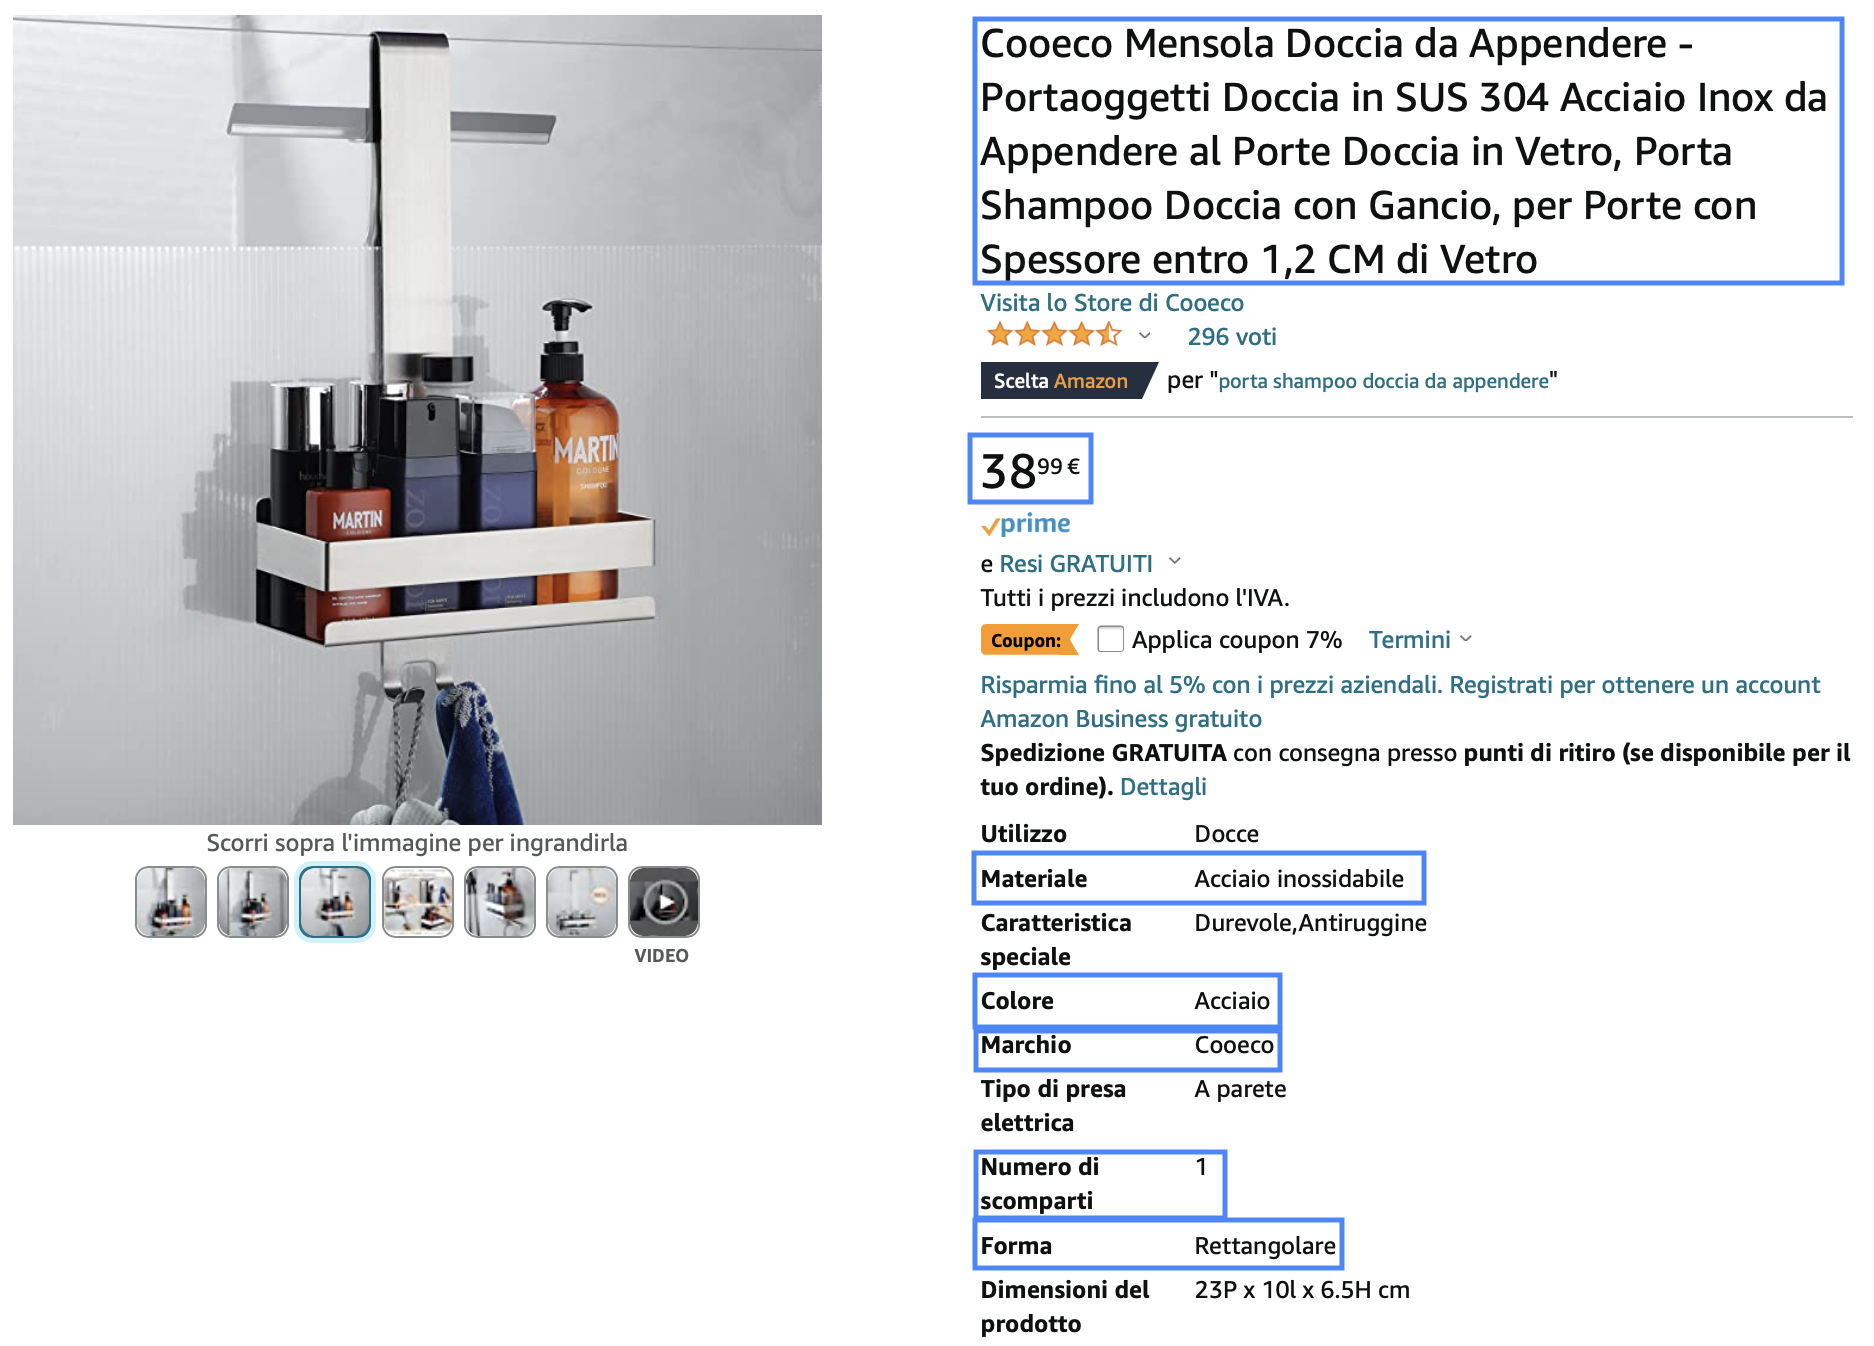
\includegraphics[scale=0.36]{img/feature.png}
    \caption{Esempio strutturale di una pagina web da cui sono state indviduate ed estratte le caratteristiche inquadrate}
    \label{fig:features}
\end{figure}

\section{Web scraping}
Il passo successivo è stato quello di trovare delle espressioni con cui soddisfare la necessità informativa. Quindi per ogni caratteristica è stata scritta un'espressione e, di conseguenza, ne è stata valutata l'efficacia, così da modificare quelle espressioni che non riportavano i risultati sperati.

Di seguito, si illustrerà come gli eventuali problemi incontrati sono stati risolti.

\subsection{Nome del prodotto}
La prima caratteristica ricercata è il nome del prodotto. 

Come visibile in figura \ref{fig:features}, esso si localizza all'inizio della pagina relativa al prodotto, questa posizione risulta essere la stessa in tutte le pagine ma, essendoci la possibilità che un banner pubblicitario alteri la struttura della stessa, si è pensato di individuare delle caratteristiche del tag, contentente il dato, che permettessero di svincolarsi dalla struttura stessa della pagina. Si è fatto leva su un tipo di attributo cui valore è standardizzato, permettendo così di individuare univocamente il tag in questione. L'attributo del tag \texttt{<span>} di cui si sta parlando è l'\texttt{id}, mentre \texttt{productTitle} è il suo valore.

\textbf{Espressione XPath}: \verb|$x("//span[@id='productTitle']/text()")|

\subsection{Prezzo prodotto}

Questa caratteristica è risultata problematica sin da subito poiché, in ogni pagina, questo dato è ridondante e presente in più posizioni all'interno della struttura html. Di conseguenza è stata scelta l'opzione migliore, che ha previsto la selezione del prezzo sottostante il nome del prodotto.

\begin{figure}[h]
    \centering
    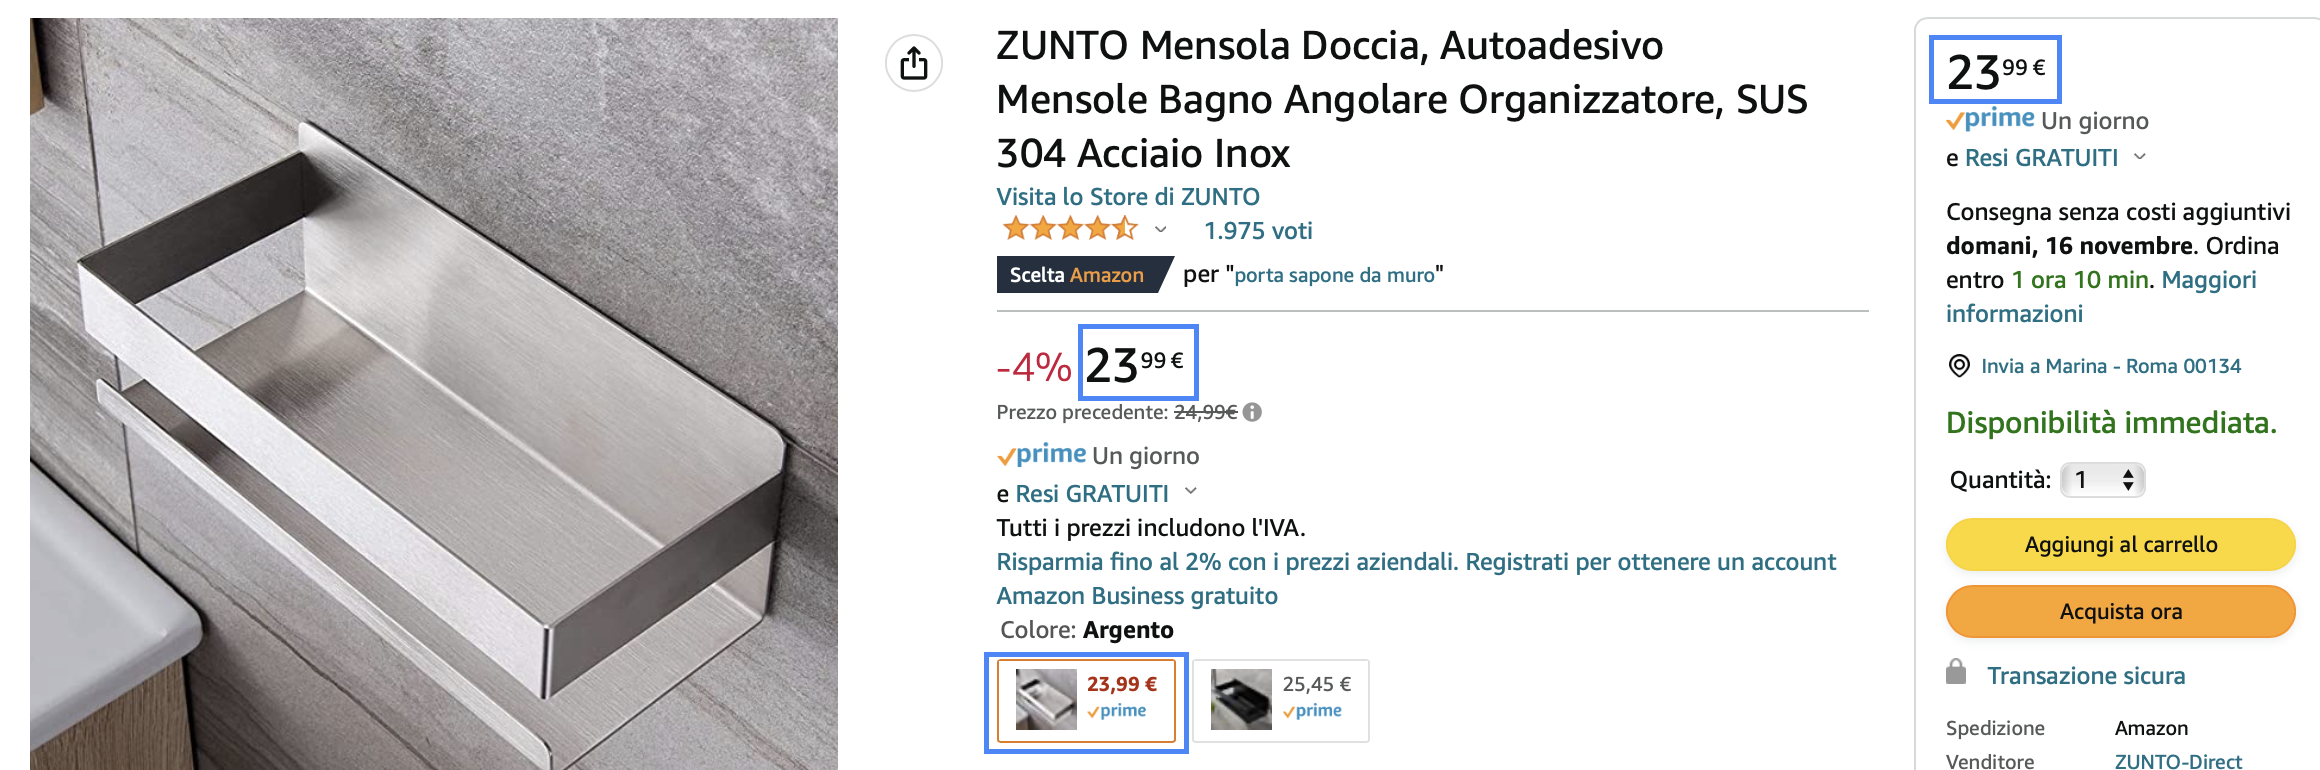
\includegraphics[width=\textwidth]{img/prezzi.png}
    \caption{lo stesso prezzo si presenta in regioni diverse}
    \label{fig:prezzi}
\end{figure}

Per farlo è stata utilizzata la seguente espressione:

\begin{verbatim}
    $x("//div[@id='apex_desktop_newAccordionRow']
        /div[@id='corePriceDisplay_desktop_feature_div']
        /div/span/span[contains(@class, 'a-offscreen')]/text()")
\end{verbatim}

Quest'ultima è risultata problematica, poiché nel secondo prodotto non veniva estratto il dato corretto. La motivazione è relativa alla forte dipendenza della soluzione adottata con la struttura della prima pagina web. Quindi è stata cercata un espressione più generale:

\begin{verbatim}
    $x("//div[@id='apex_desktop']
        /descendant::div[@id='corePriceDisplay_desktop_feature_div']
        /descendant::span[contains(@class, 'a-offscreen')]/text()")
\end{verbatim}

L'array riportato in questo caso, risulta essere parzialmente corretto a causa dei due prezzi che lo compongono. In particolare, il primo rappresenta il prezzo che si vuole estrarre, mentre il secondo, dopo un'attenta analisi, si osserva essere invisibile nella pagina, probabilmente nascosto per qualche motivo. Questa anomalia era condivisa da pochi altri prodotti, dunque 
% Ma questo prezzo non viene visualizzato da nessuna parte quindi è stato ipotizzato che fosse un prezzo nascosto nella pagina html, quindi è stato ricercato un tag contentente uno stile associato ad un css. L'assunzione che è stata fatta prevedeva che esso fosse visibile grazie a questo tipo di file.
% \begin{verbatim}
%     $x("//div[@id='apex_desktop']
%         /descendant::div[@id='corePriceDisplay_desktop_feature_div']
%         /style[contains(@type, 'text/css')]
%         /following-sibling::div
%         /descendant::span[contains(@class, 'a-offscreen')]/text()")
% \end{verbatim}
è stato preso il primo riportato poiché sempre coincidente con il prezzo mostrato a schermo:

\begin{verbatim}
    $x("(//div[@id='corePriceDisplay_desktop_feature_div']
        //span[contains(@class,'a-offscreen')])[1]/text()")
\end{verbatim}

Da notare che questa espressione è stata considerata corretta per il prodotto \ref{it:prod3}, in cui è presente un ulteriore prezzo di cui non viene fatto il display, ma viene mantenuto nascosto per agevolare un'animazione che ha luogo qualora l'utente scelga di usufruire della prova gratuito del prodotto.

\subsection{Altre caratteristiche}
Le altre caratteristiche scelte, sono presenti in una forma tabellare facilmente accessibile tramite espressioni \textit{XPath}. Questa tabella html prevede che il valore di una caratteristica sia subito dopo il nome della stessa. Di conseguenza si è pensato di individuare il tag cui testo coincide con il nome della caratteristica, per poi estrarre il valore associato prendendo lo \texttt{<span>} a fianco. Questo ragionamento è stato ripetuto per tutte le altre caratteristiche scelte (vedi \ref{it:features}): inizialmente sono state provate delle espressioni che prevedevano questo tipo ricerca: \verb|//...[text()='Materiale']/.../text()|.

Si noti però, che questa scelta non è stata ottimale per la "Forma" dei prodotti, poiché 
il valore testuale nei nodi è risultato, a volte, contenere caratteri che apparentemente sembrano spazi bianchi, ma che in realtà non lo sono. 

Quindi, l'uso dell'uguaglianza è risultato meno efficace rispetto ad espressioni del tipo \verb|contains(<h>, <valore che deve essere contenuto in h>)|. 

Un esempio è il seguente:
\begin{verbatim}
    $x("//span[contains(text(),'Materiale')]
        /ancestor::td/following-sibling::td/span/text()")
\end{verbatim}

\begin{figure}[h]
    \centering
    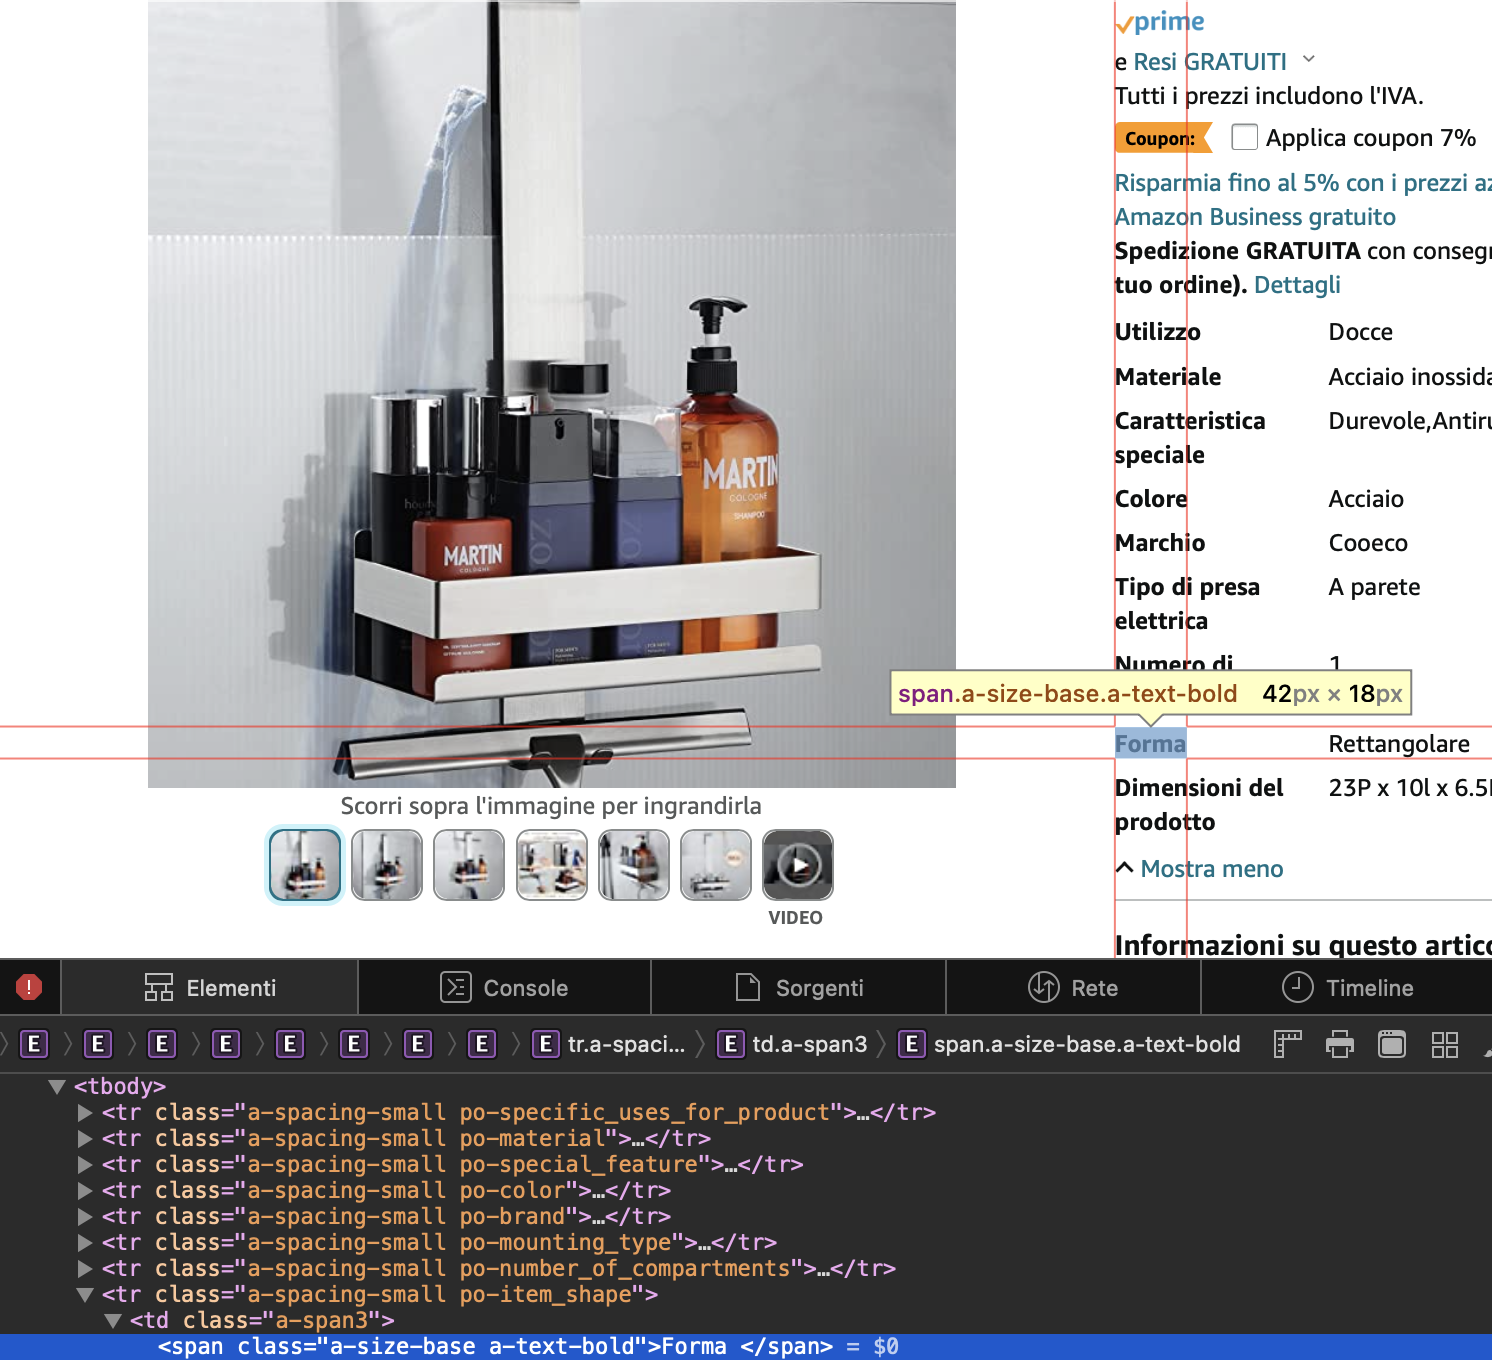
\includegraphics[width=\textwidth]{img/forma_problem.png}
    \caption{Nel tag \texttt{<span>} evidenziato, la stringa "Forma" è seguita da caratteri speciali diversi dallo spazio bianco}
    \label{fig:my_label}
\end{figure}

\newpage
Successivamente, sono stati notati degli attributi contenenti valori relativi alle caratteristiche cercate (e.g. \verb|class='po-material'| per il "Materiale"), cui utilizzo ha permesso, inoltre, indipendenza dal testo scritto e quindi dalla lingua utilizzata nel sito.

Di seguito le espressioni che sono state utilizzate:
\begin{table}[h]
    \begin{tabularx}{\textwidth}{|X|}
        \hline
        \textbf{Materiale} \\
        \hline
        \verb|$x("//tr[contains(@class,'po-material')]|
        \newline
        \verb|/td[contains(@class,'a-span9')]/span/text()")|\\
        \hline
    \end{tabularx}
\label{tab:my_label}
\end{table}
\begin{table}[h]
    \begin{tabularx}{\textwidth}{|X|}
        \hline
        \textbf{Colore} \\
        \hline
        \verb|$x("//tr[contains(@class,'po-color')]|
        \newline
        \verb|/td[contains(@class,'a-span9')]/span/text()")|\\
        \hline
    \end{tabularx}
\label{tab:my_label}
\end{table}
\begin{table}[h]
    \begin{tabularx}{\textwidth}{|X|}
        \hline
        \textbf{Marchio} \\
        \hline
        \verb|$x("//tr[contains(@class,'po-brand')]|
        \newline
        \verb|/td[contains(@class,'a-span9')]/span/text()")|\\
        \hline
    \end{tabularx}
\label{tab:my_label}
\end{table}
\begin{table}[h]
    \begin{tabularx}{\textwidth}{|X|}
        \hline
        \textbf{Numero di scomparti} \\
        \hline
        \verb|$x("//tr[contains(@class,'po-number_of_compartments')]|
        \newline
        \verb|/td[contains(@class,'a-span9')]/span/text()")|\\
        \hline
    \end{tabularx}
\label{tab:my_label}
\end{table}
\begin{table}[h!]
    \begin{tabularx}{\textwidth}{|X|}
        \hline
        \textbf{Forma} \\
        \hline
        \verb|$x("//tr[contains(@class,'po-item_shape')]|
        \newline
        \verb|/td[contains(@class,'a-span9')]/span/text()")|\\
        \hline
    \end{tabularx}
\label{tab:my_label}
\end{table}
\newpage
Si noti che alcune di queste caratteristiche non sono presenti in alcune pagine, quindi sono ritornati array vuoti.

% \section{Risultati}
% \subsection{Primo prodotto}
% \begin{figure}[h]
%     \centering
%     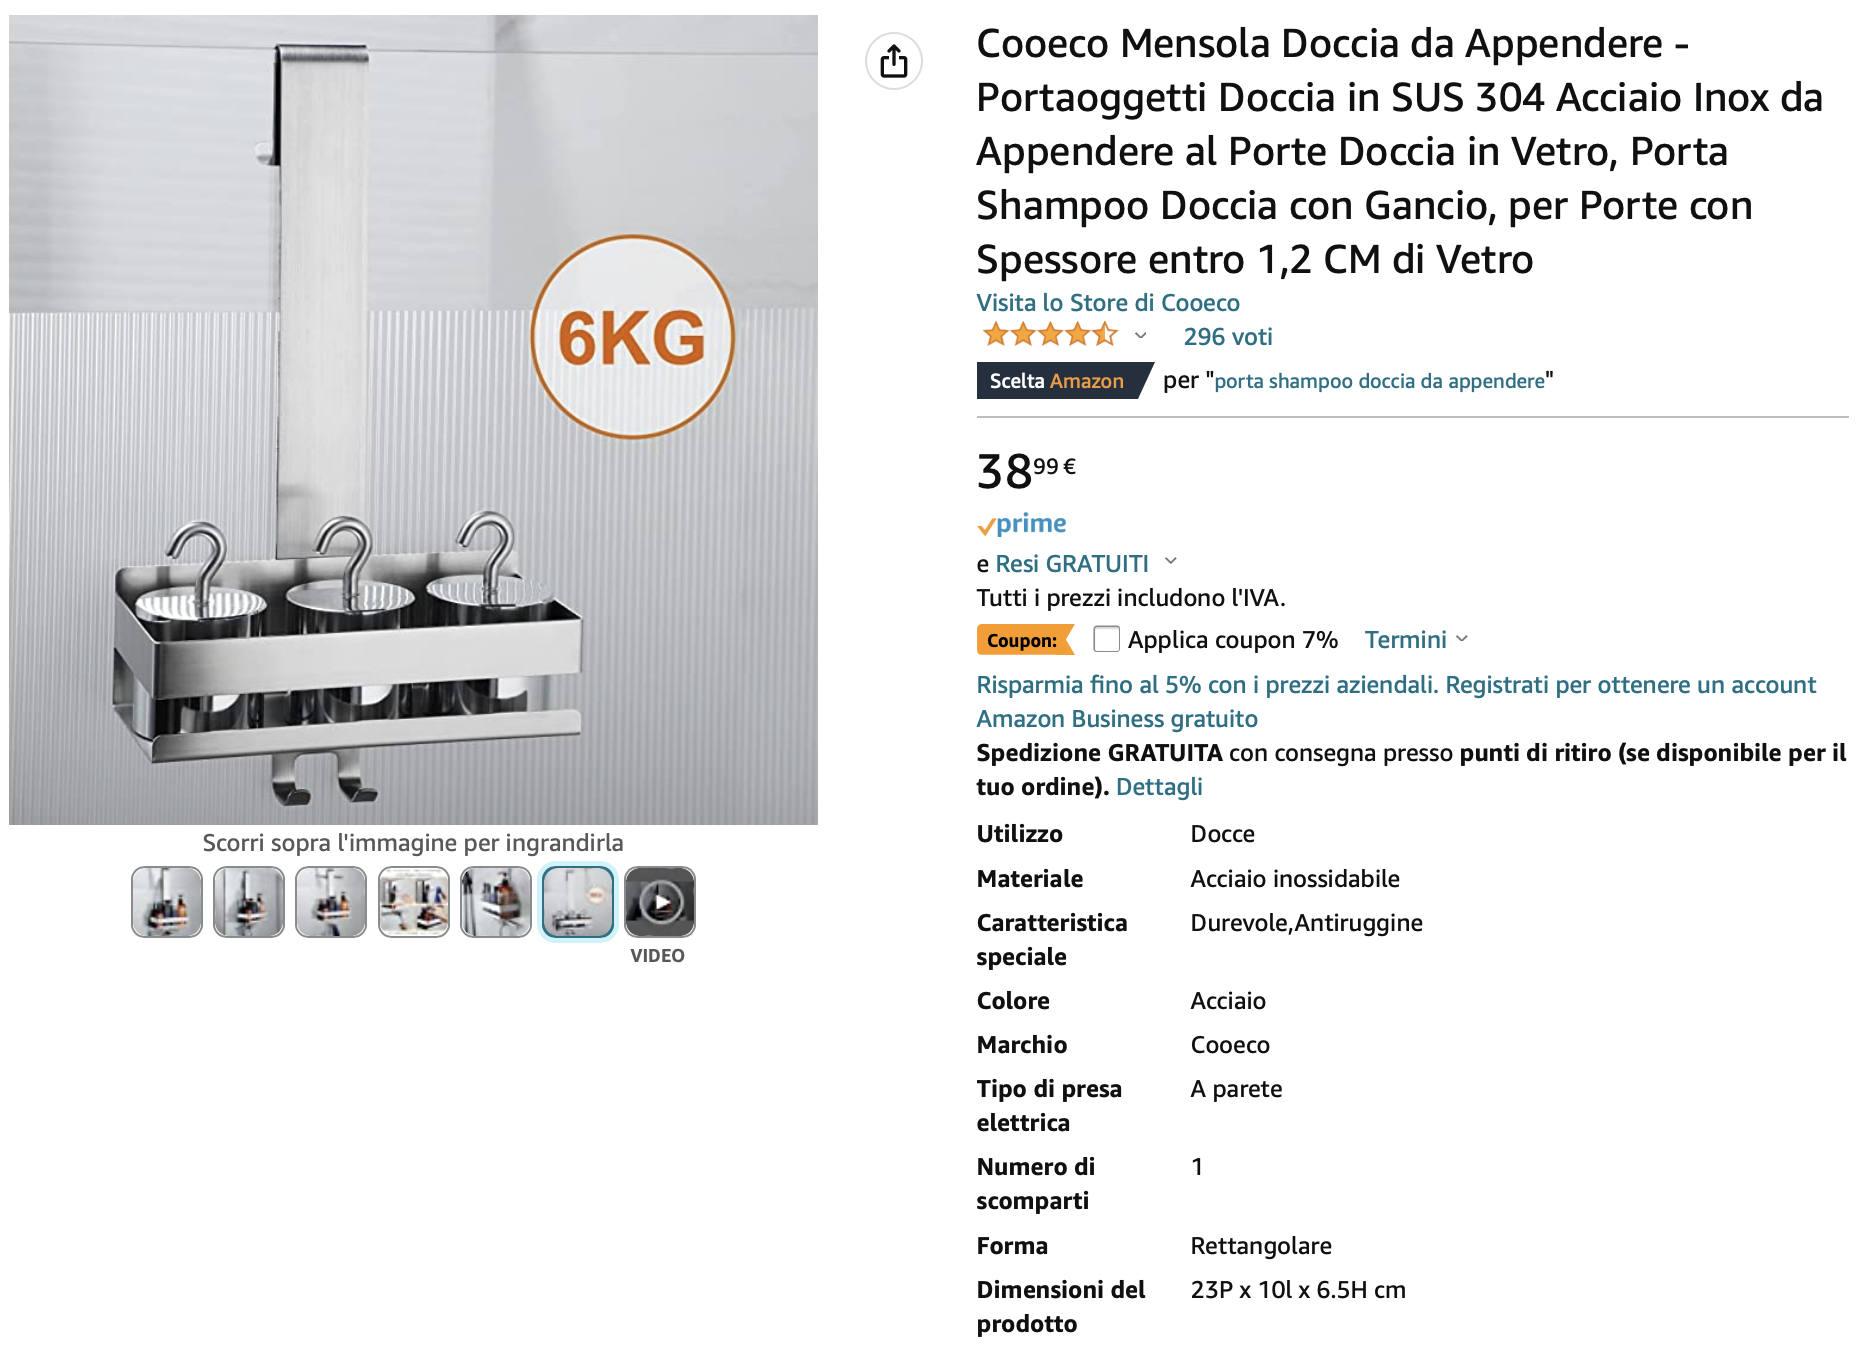
\includegraphics[width=\textwidth, scale=0.2]{img/prod1.png}
%     \caption{Caption}
%     \label{fig:my_label}
% \end{figure}
% \begin{table}[h]
%     \begin{tabular}{|c|c|}
%         \hline
%         \textbf{Materiale} & \\
%         \hline
%         \textbf{Colore} & \\
%         \hline
%         \textbf{Marchio} & \\
%         \hline
%         \textbf{Numero di scomparti} & \\
%         \hline
%         \textbf{Forma} & \\
%         \hline
%     \end{tabular}
%     \caption{Espressioni usate per le restanti caratteristiche}
%     \label{tab:my_label}
% \end{table}

% \subsection{Secondo prodotto}
% \begin{figure}[h]
%     \centering
%     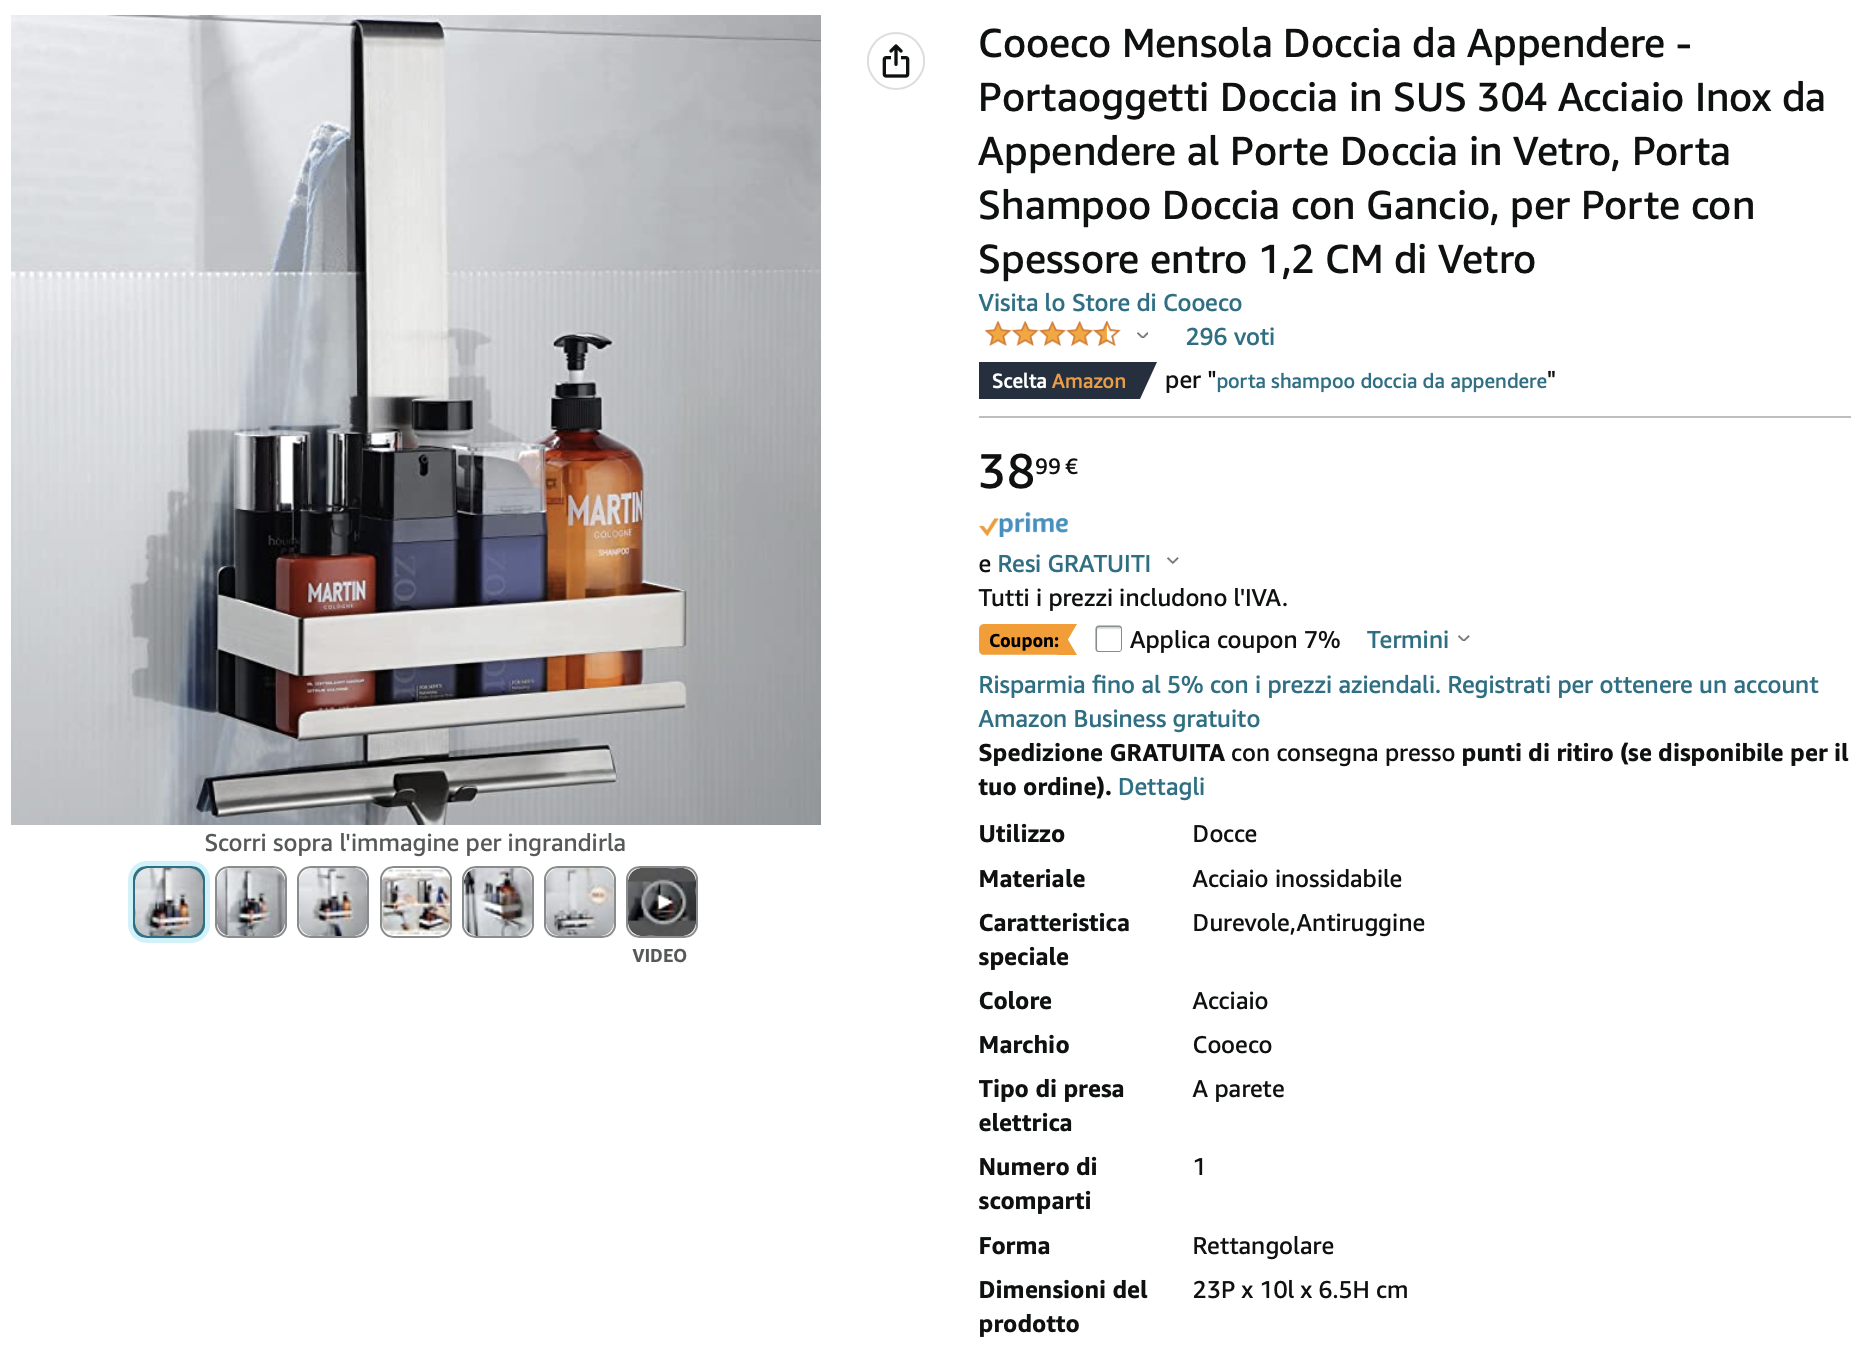
\includegraphics[width=\textwidth, scale=0.2]{img/prod2.png}
%     \caption{Caption}
%     \label{fig:my_label}
% \end{figure}
% \begin{table}[h]
%     \begin{tabular}{|c|c|}
%         \hline
%         \textbf{Materiale} & \\
%         \hline
%         \textbf{Colore} & \\
%         \hline
%         \textbf{Marchio} & \\
%         \hline
%         \textbf{Numero di scomparti} & \\
%         \hline
%         \textbf{Forma} & \\
%         \hline
%     \end{tabular}
%     \caption{Espressioni usate per le restanti caratteristiche}
%     \label{tab:my_label}
% \end{table}

% \subsection{Terzo prodotto}
% \begin{figure}[h]
%     \centering
%     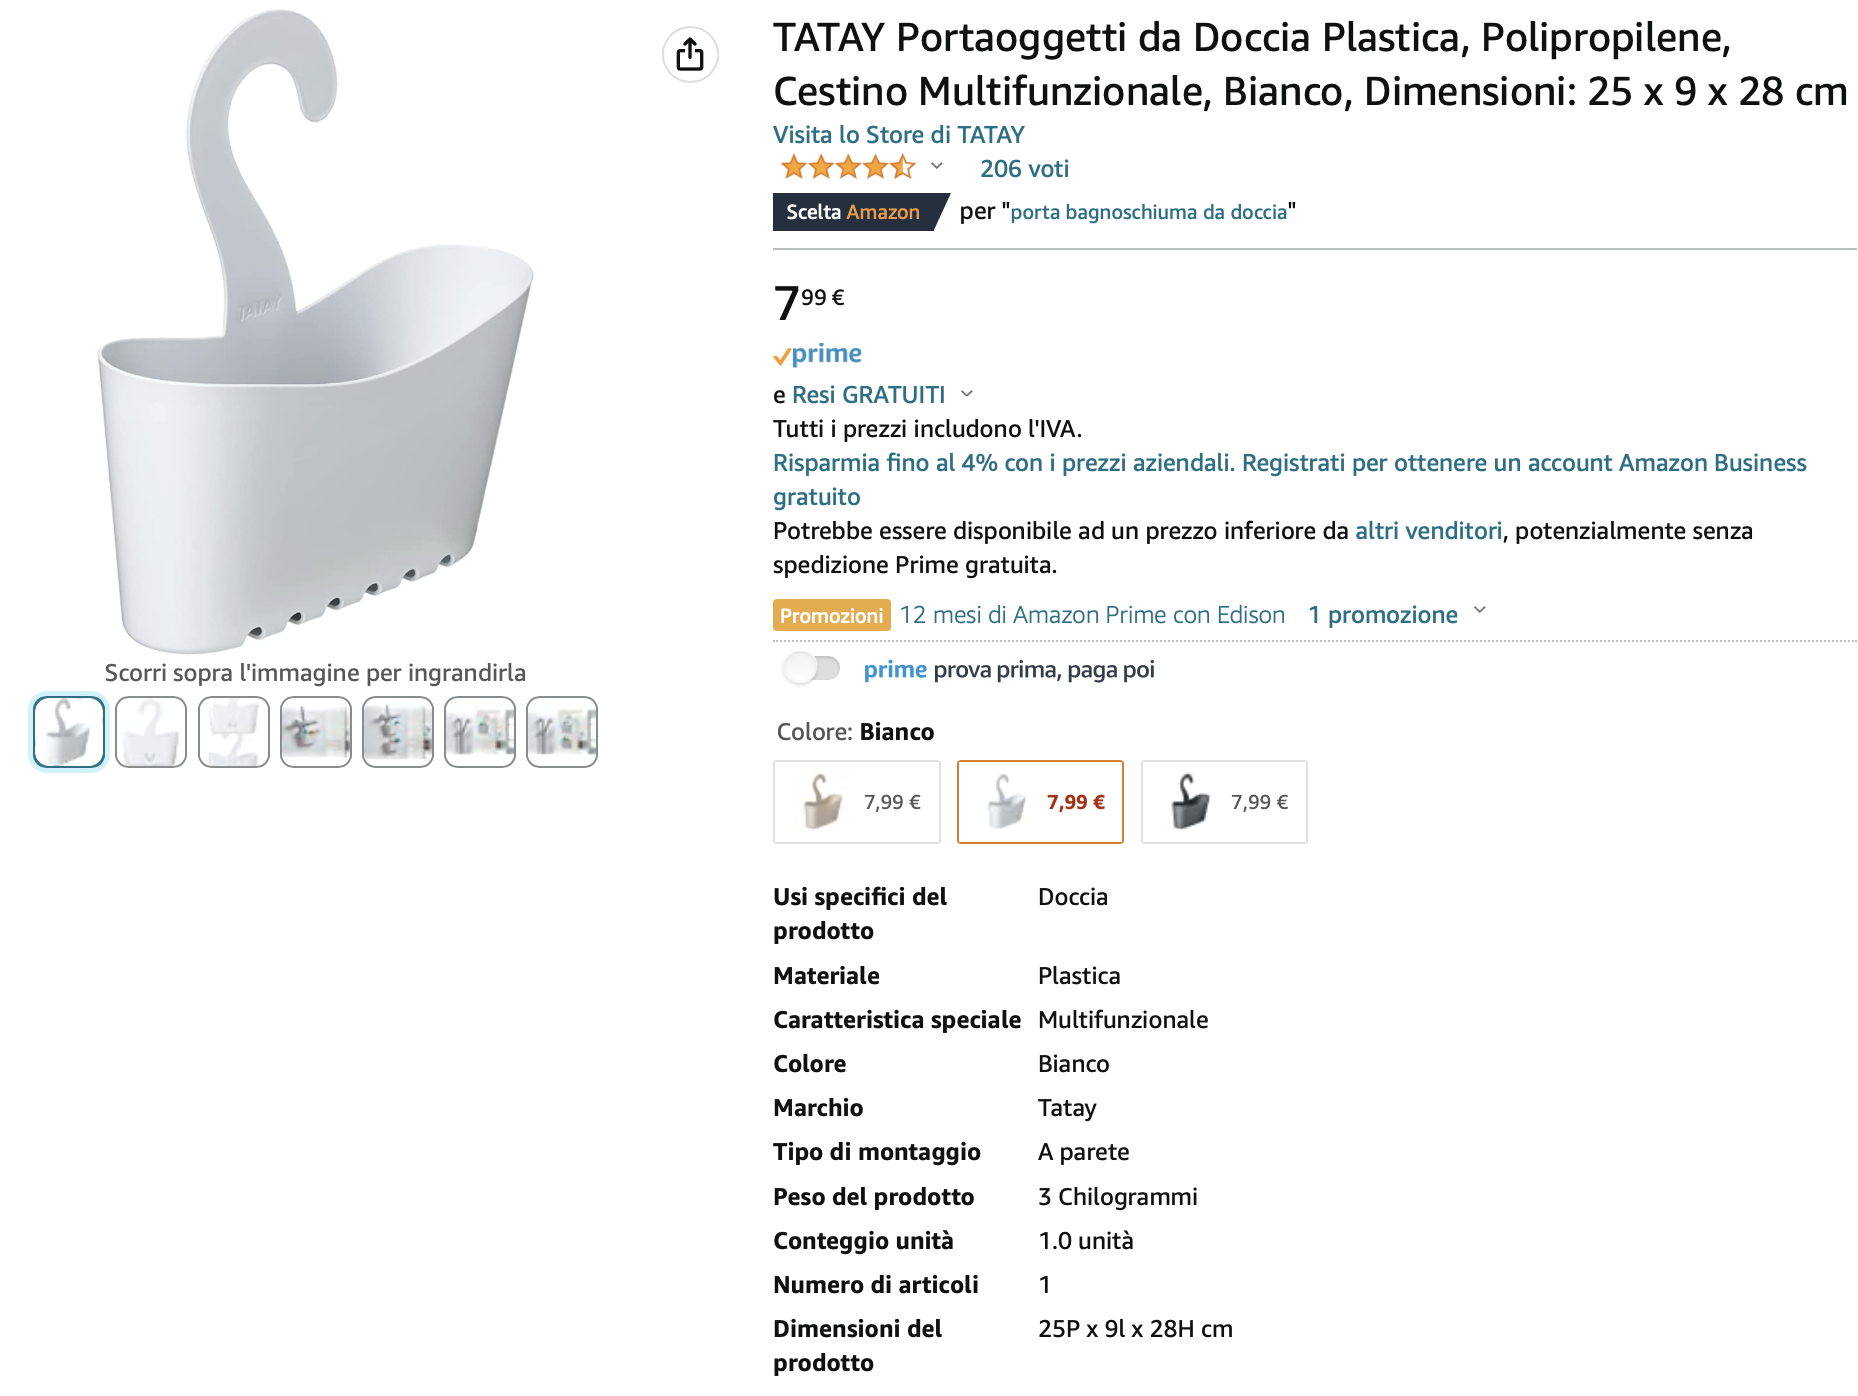
\includegraphics[width=\textwidth, scale=0.2]{img/prod3.png}
%     \caption{Caption}
%     \label{fig:my_label}
% \end{figure}
% \begin{table}[h]
%     \begin{tabular}{|c|c|}
%         \hline
%         \textbf{Materiale} & \\
%         \hline
%         \textbf{Colore} & \\
%         \hline
%         \textbf{Marchio} & \\
%         \hline
%         \textbf{Numero di scomparti} & \\
%         \hline
%         \textbf{Forma} & \\
%         \hline
%     \end{tabular}
%     \caption{Espressioni usate per le restanti caratteristiche}
%     \label{tab:my_label}
% \end{table}

% \subsection{Quarto prodotto}
% \begin{figure}[h]
%     \centering
%     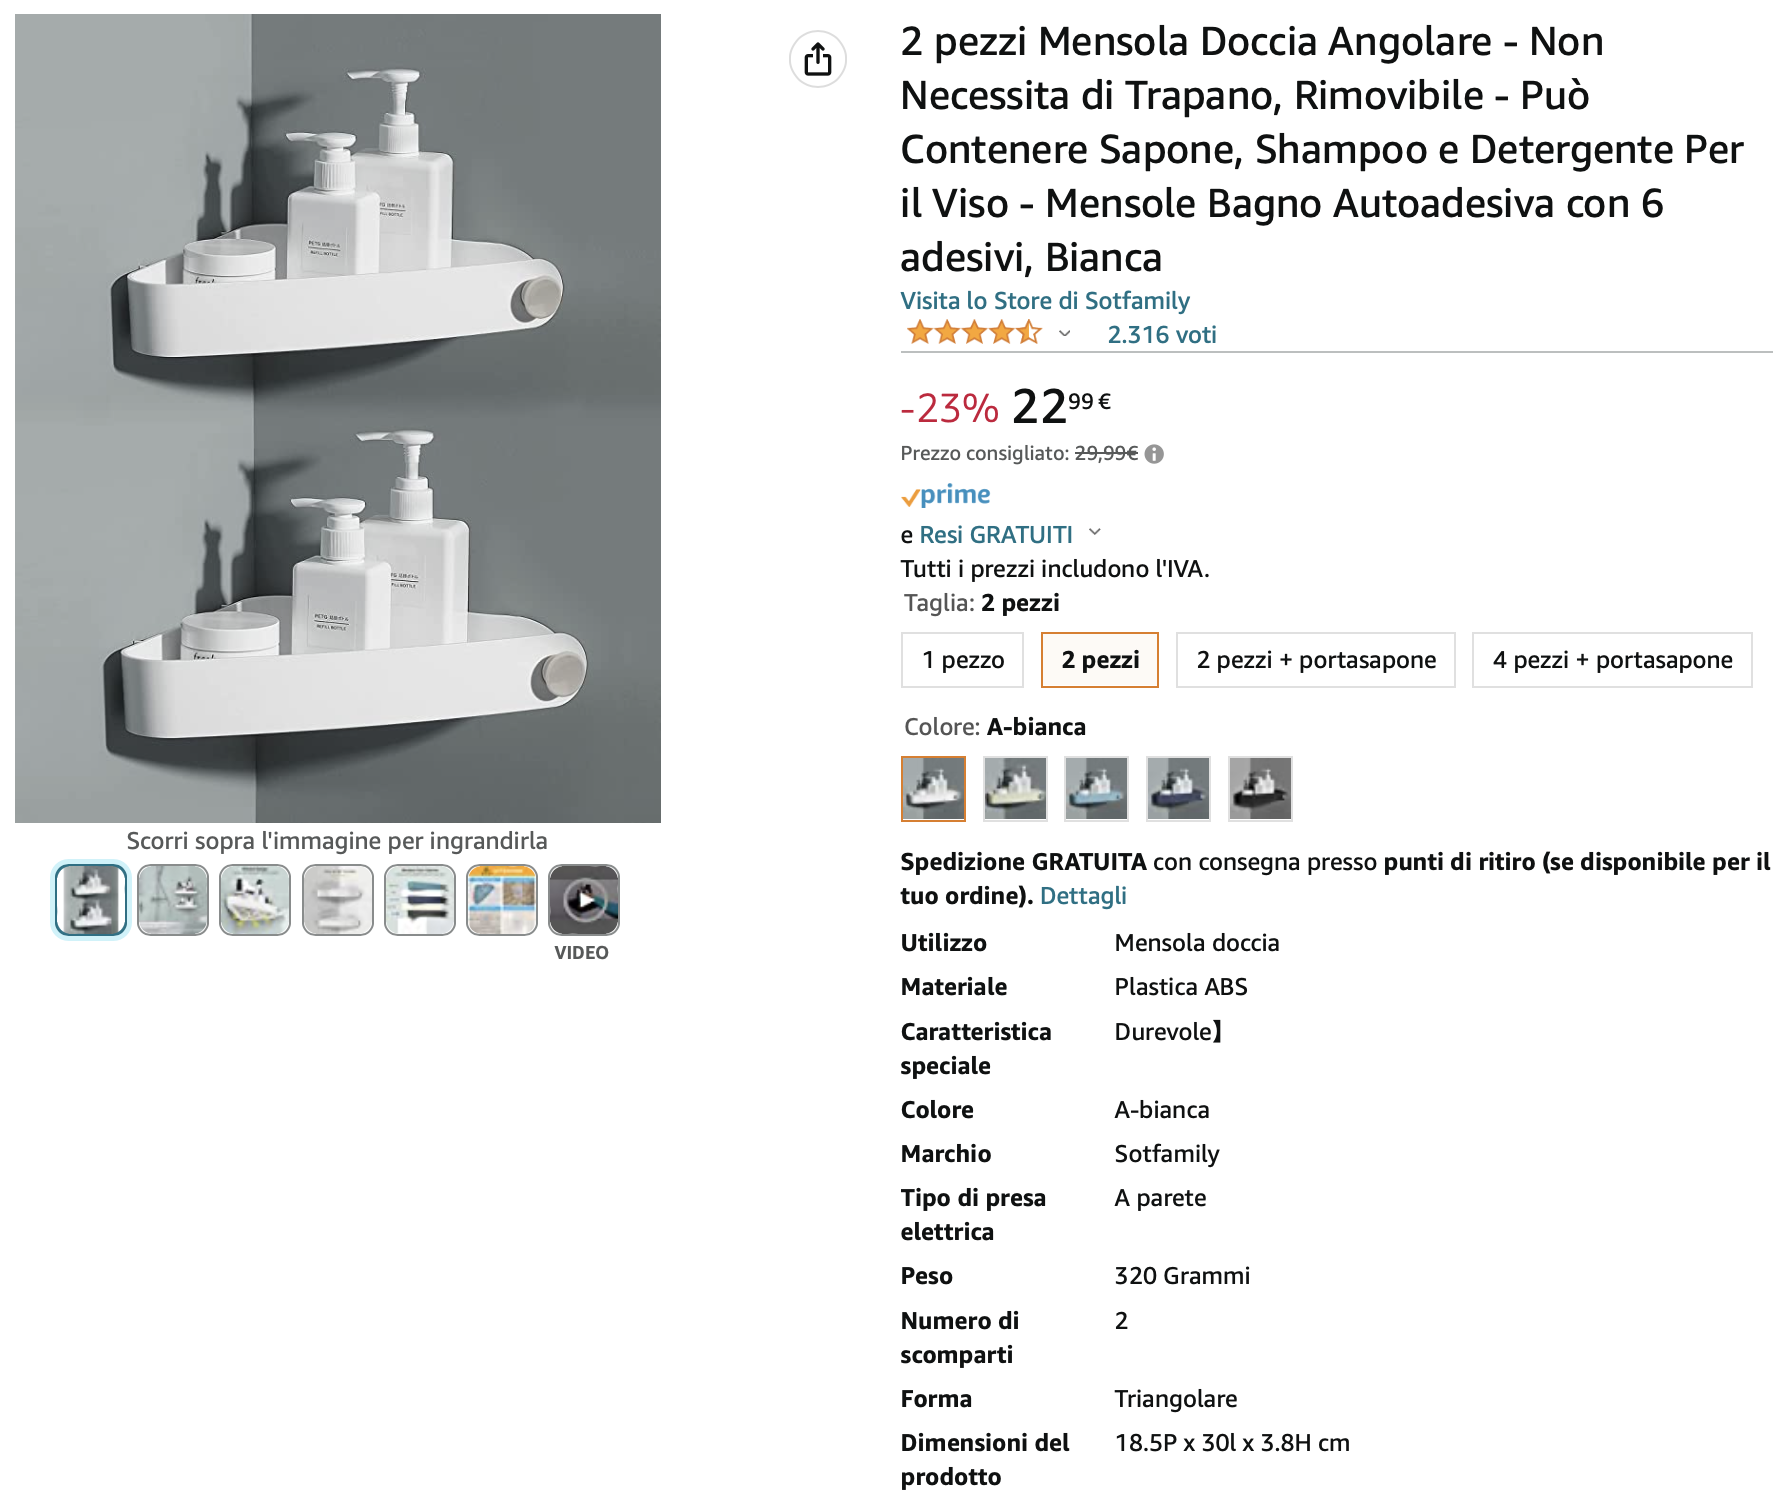
\includegraphics[width=\textwidth, scale=0.2]{img/prod4.png}
%     \caption{Caption}
%     \label{fig:my_label}
% \end{figure}
% \begin{table}[h]
%     \begin{tabular}{|c|c|}
%         \hline
%         \textbf{Materiale} & \\
%         \hline
%         \textbf{Colore} & \\
%         \hline
%         \textbf{Marchio} & \\
%         \hline
%         \textbf{Numero di scomparti} & \\
%         \hline
%         \textbf{Forma} & \\
%         \hline
%     \end{tabular}
%     \caption{Espressioni usate per le restanti caratteristiche}
%     \label{tab:my_label}
% \end{table}

% \subsection{Quinto prodotto}
% \begin{figure}[h]
%     \centering
%     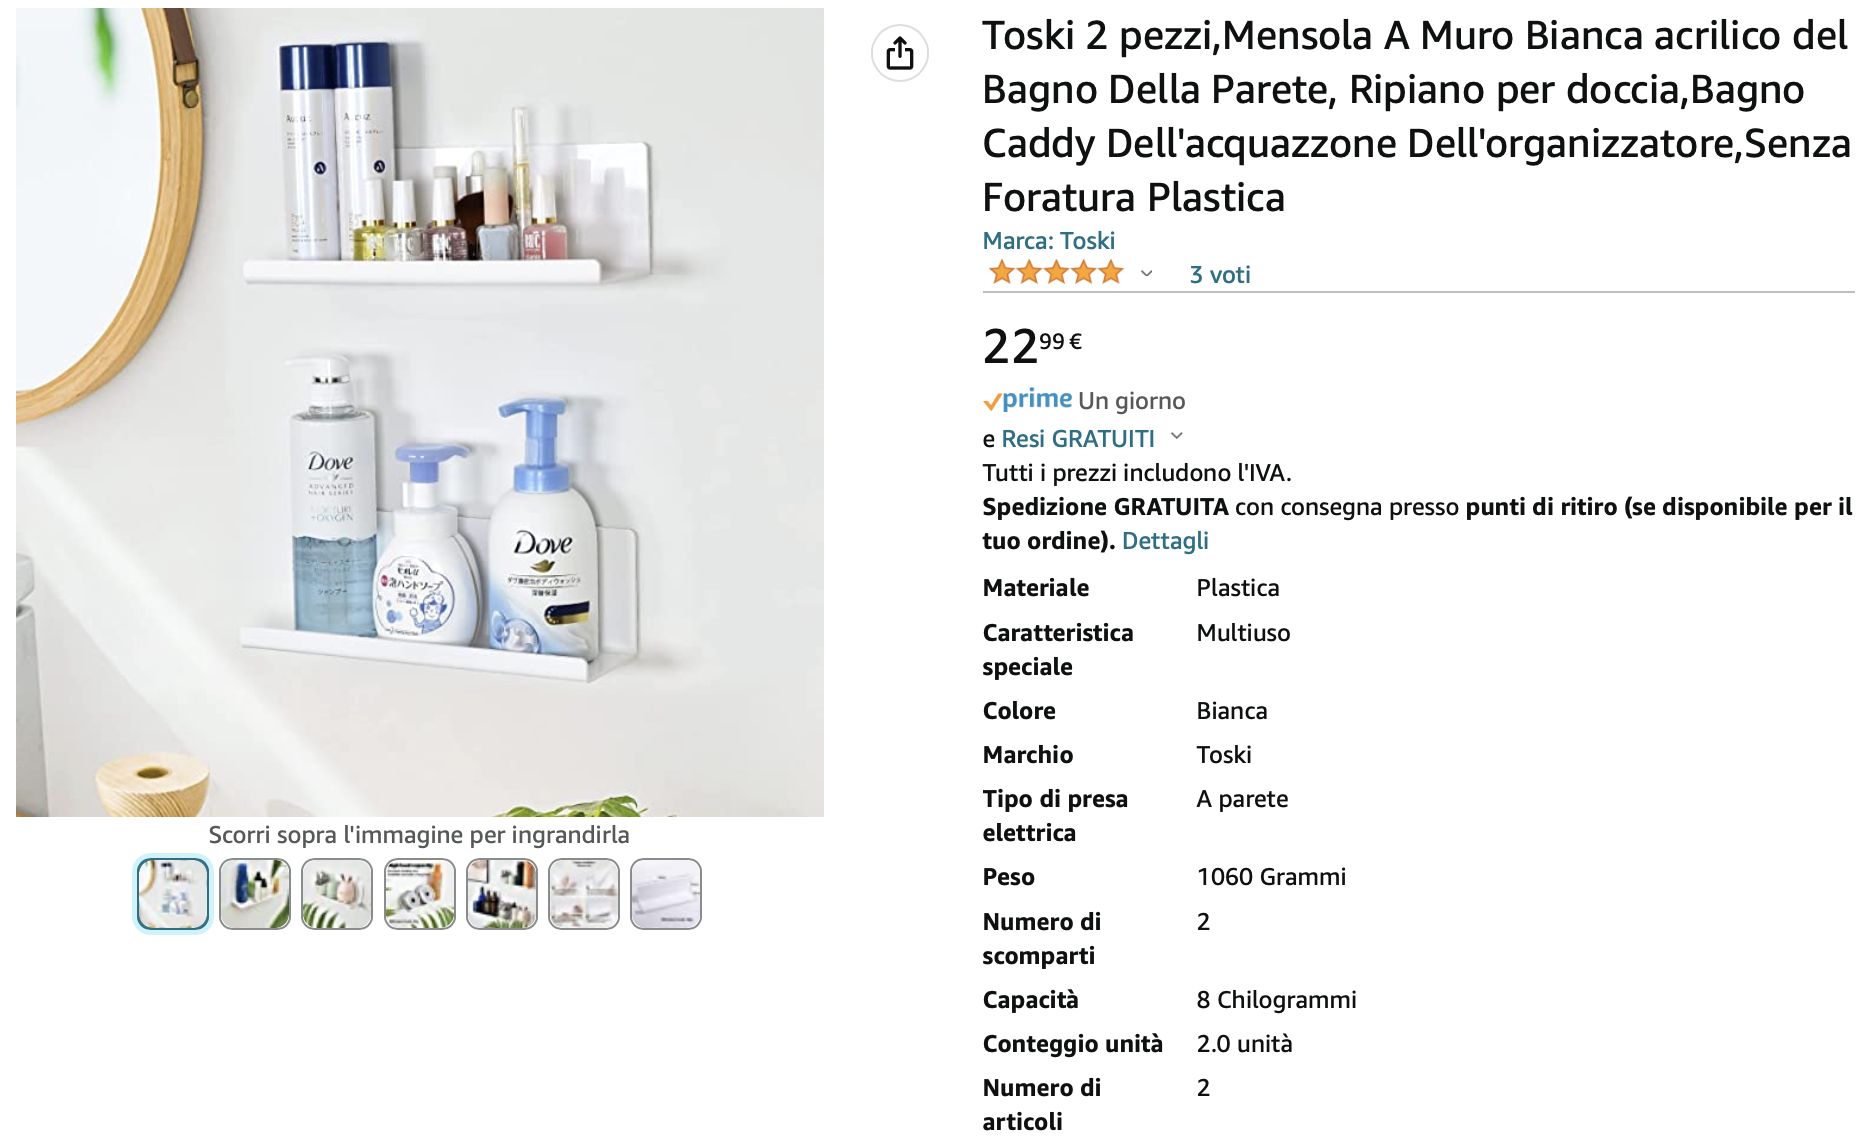
\includegraphics[width=\textwidth, scale=0.2]{img/prod5.png}
%     \caption{Caption}
%     \label{fig:my_label}
% \end{figure}
% \begin{table}[h]
%     \begin{tabular}{|c|c|}
%         \hline
%         \textbf{Materiale} & \\
%         \hline
%         \textbf{Colore} & \\
%         \hline
%         \textbf{Marchio} & \\
%         \hline
%         \textbf{Numero di scomparti} & \\
%         \hline
%         \textbf{Forma} & \\
%         \hline
%     \end{tabular}
%     \caption{Espressioni usate per le restanti caratteristiche}
%     \label{tab:my_label}
% \end{table}

% \subsection{Sesto prodotto}
% \begin{figure}[h]
%     \centering
%     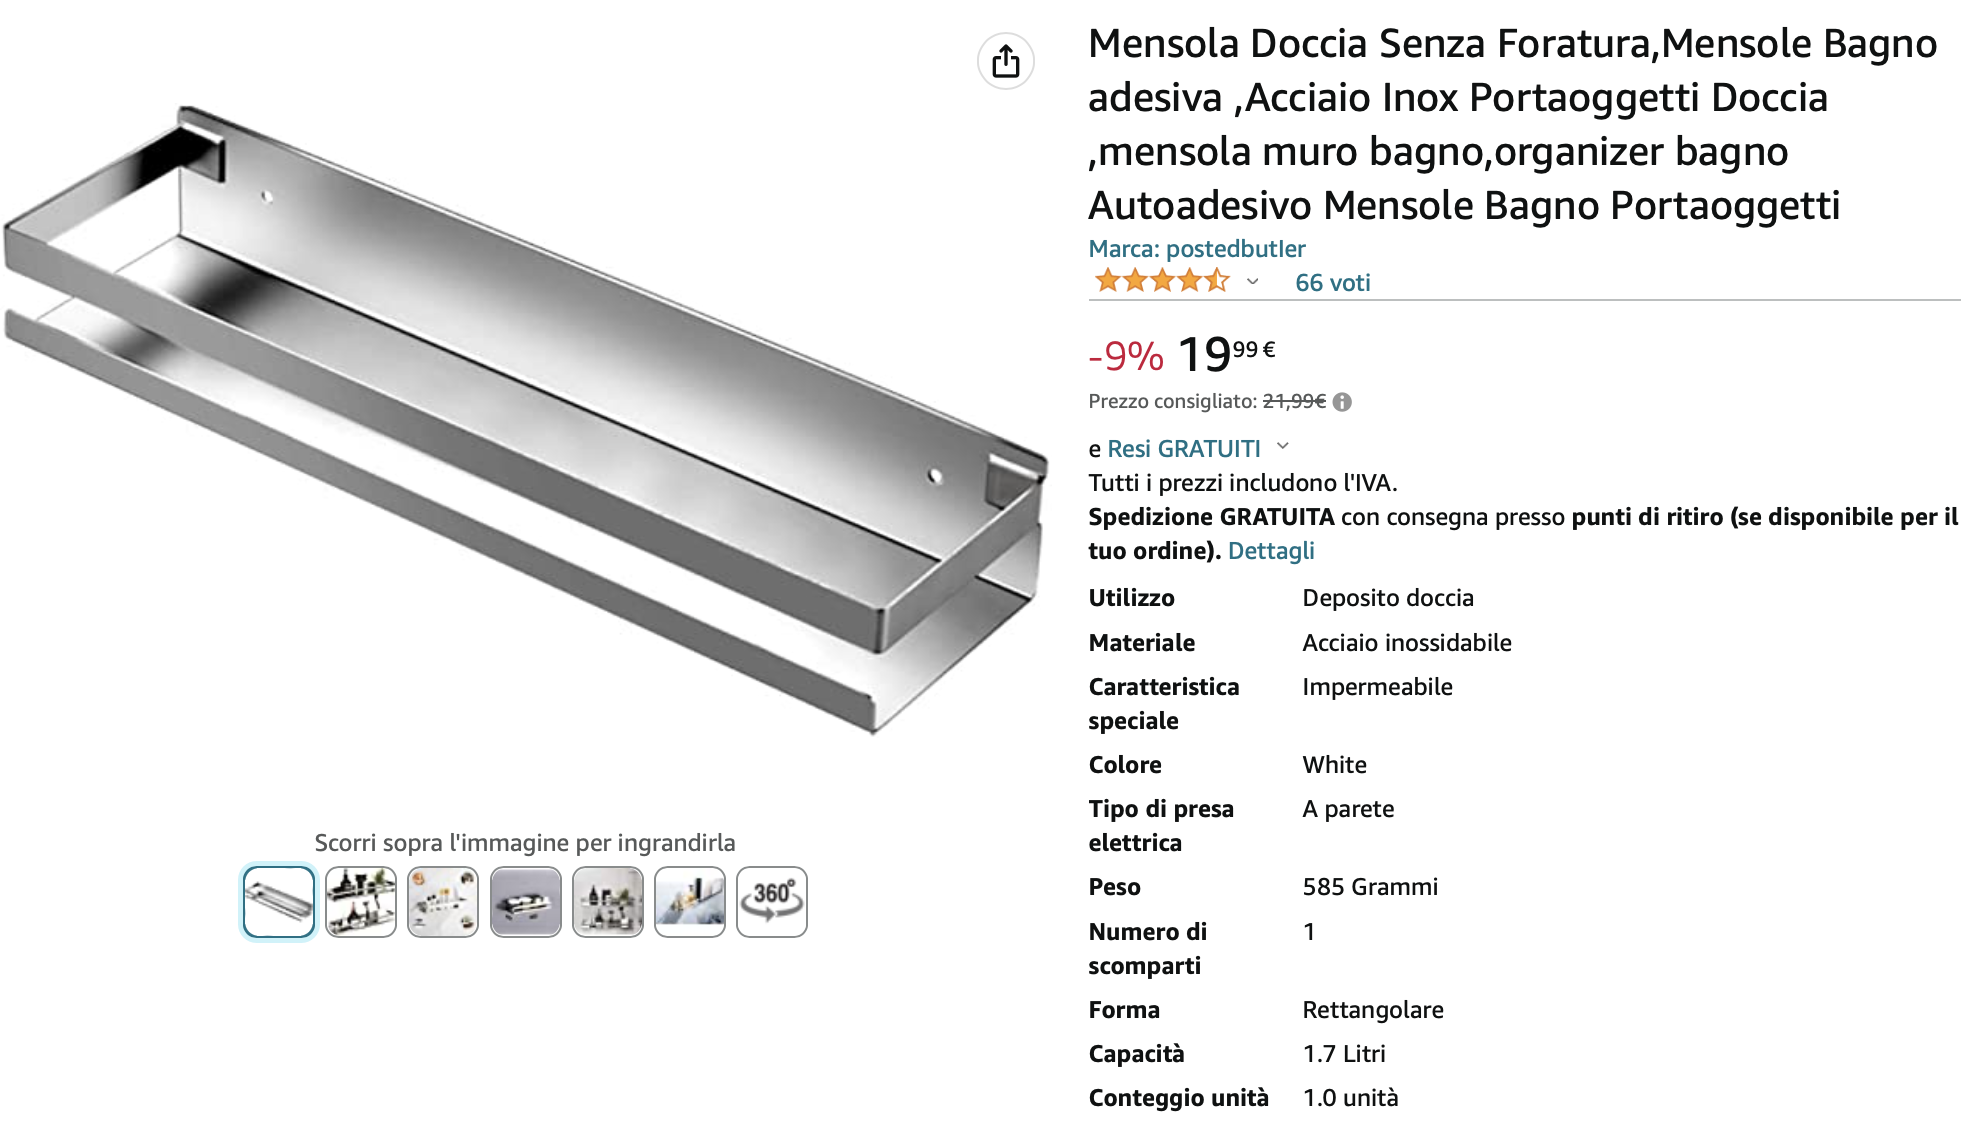
\includegraphics[width=\textwidth, scale=0.2]{img/prod6.png}
%     \caption{Caption}
%     \label{fig:my_label}
% \end{figure}
% \begin{table}[h]
%     \begin{tabular}{|c|c|}
%         \hline
%         \textbf{Materiale} & \\
%         \hline
%         \textbf{Colore} & \\
%         \hline
%         \textbf{Marchio} & \\
%         \hline
%         \textbf{Numero di scomparti} & \\
%         \hline
%         \textbf{Forma} & \\
%         \hline
%     \end{tabular}
%     \caption{Espressioni usate per le restanti caratteristiche}
%     \label{tab:my_label}
% \end{table}

% \subsection{Settimo prodotto}
% \begin{figure}[h]
%     \centering
%     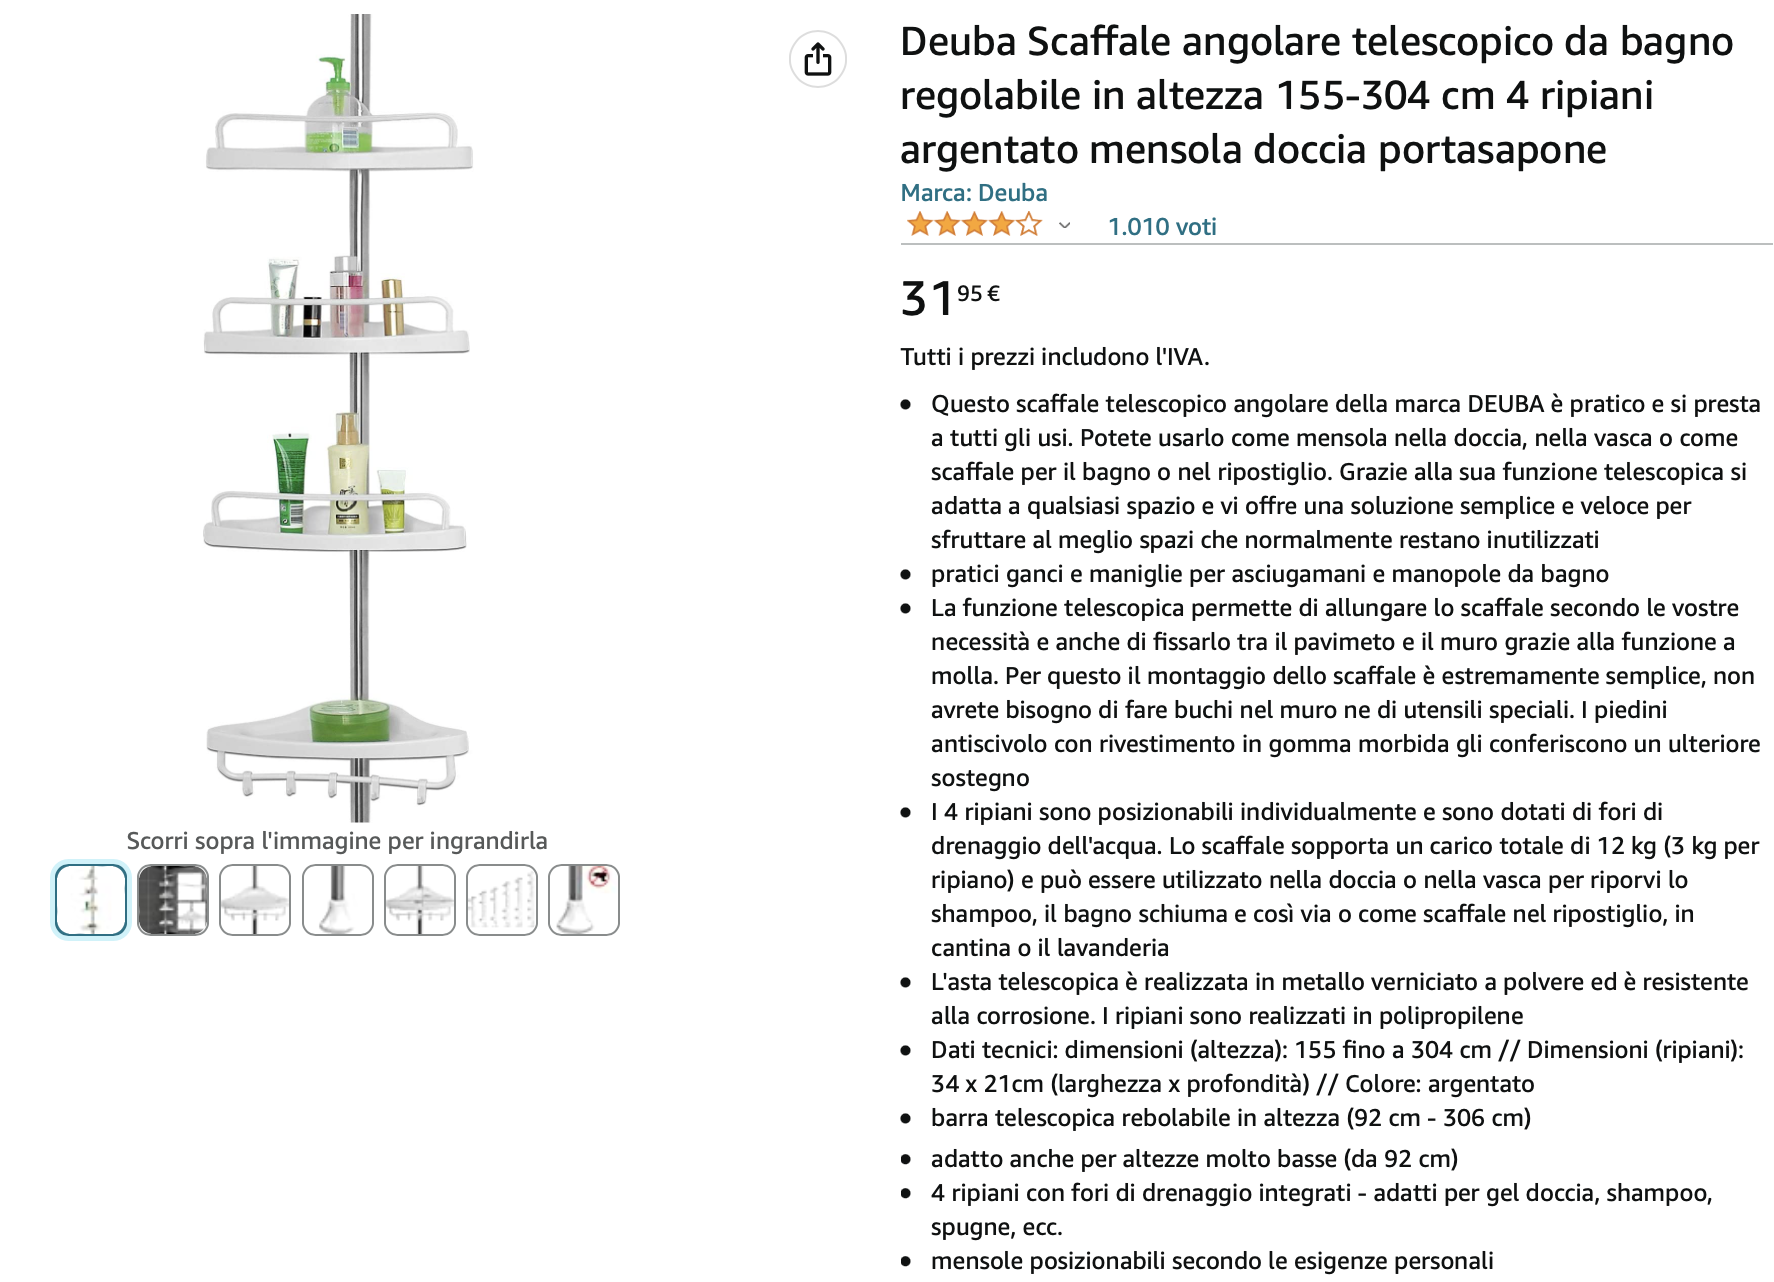
\includegraphics[width=\textwidth, scale=0.2]{img/prod7.png}
%     \caption{Caption}
%     \label{fig:my_label}
% \end{figure}
% \begin{table}[h]
%     \begin{tabular}{|c|c|}
%         \hline
%         \textbf{Materiale} & \\
%         \hline
%         \textbf{Colore} & \\
%         \hline
%         \textbf{Marchio} & \\
%         \hline
%         \textbf{Numero di scomparti} & \\
%         \hline
%         \textbf{Forma} & \\
%         \hline
%     \end{tabular}
%     \caption{Espressioni usate per le restanti caratteristiche}
%     \label{tab:my_label}
% \end{table}

% \subsection{Ottavo prodotto}
% \begin{figure}[h]
%     \centering
%     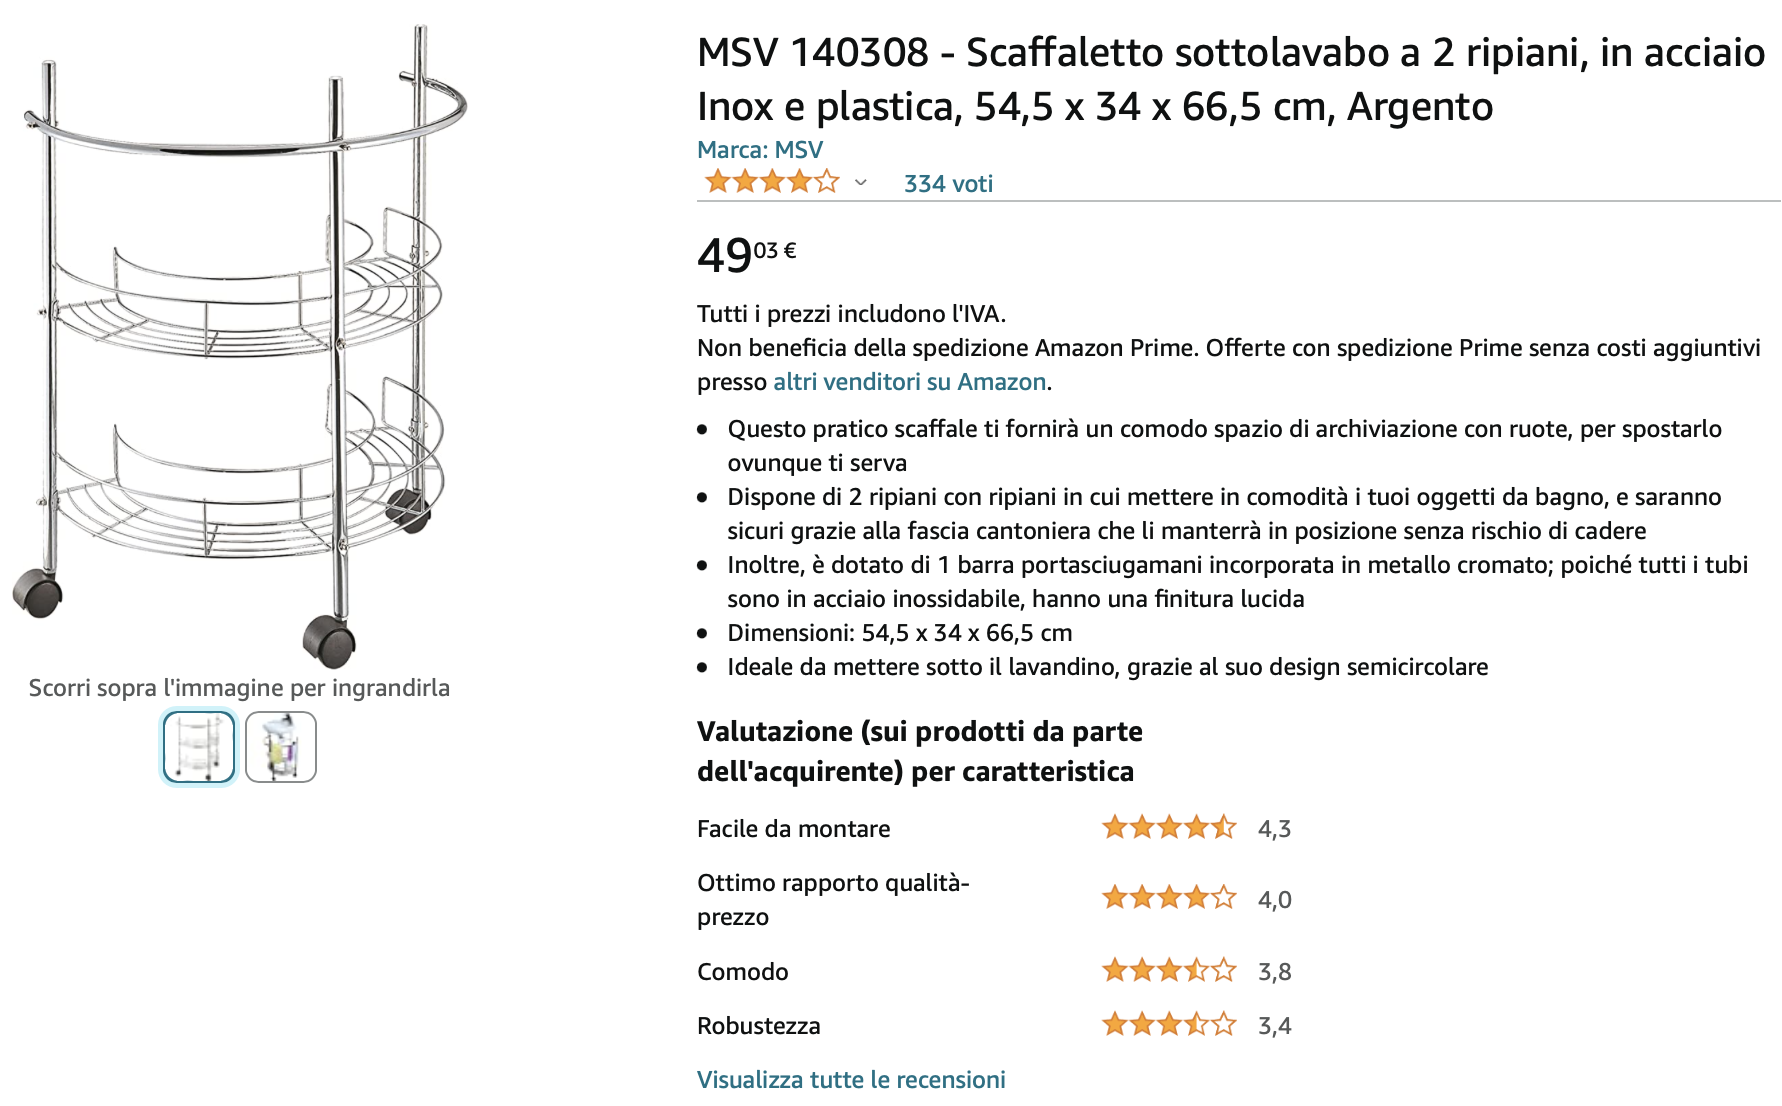
\includegraphics[width=\textwidth, scale=0.2]{img/prod8.png}
%     \caption{Caption}
%     \label{fig:my_label}
% \end{figure}
% \begin{table}[h]
%     \begin{tabular}{|c|c|}
%         \hline
%         \textbf{Materiale} & \\
%         \hline
%         \textbf{Colore} & \\
%         \hline
%         \textbf{Marchio} & \\
%         \hline
%         \textbf{Numero di scomparti} & \\
%         \hline
%         \textbf{Forma} & \\
%         \hline
%     \end{tabular}
%     \caption{Espressioni usate per le restanti caratteristiche}
%     \label{tab:my_label}
% \end{table}

% \subsection{Nono prodotto}
% \begin{figure}[h]
%     \centering
%     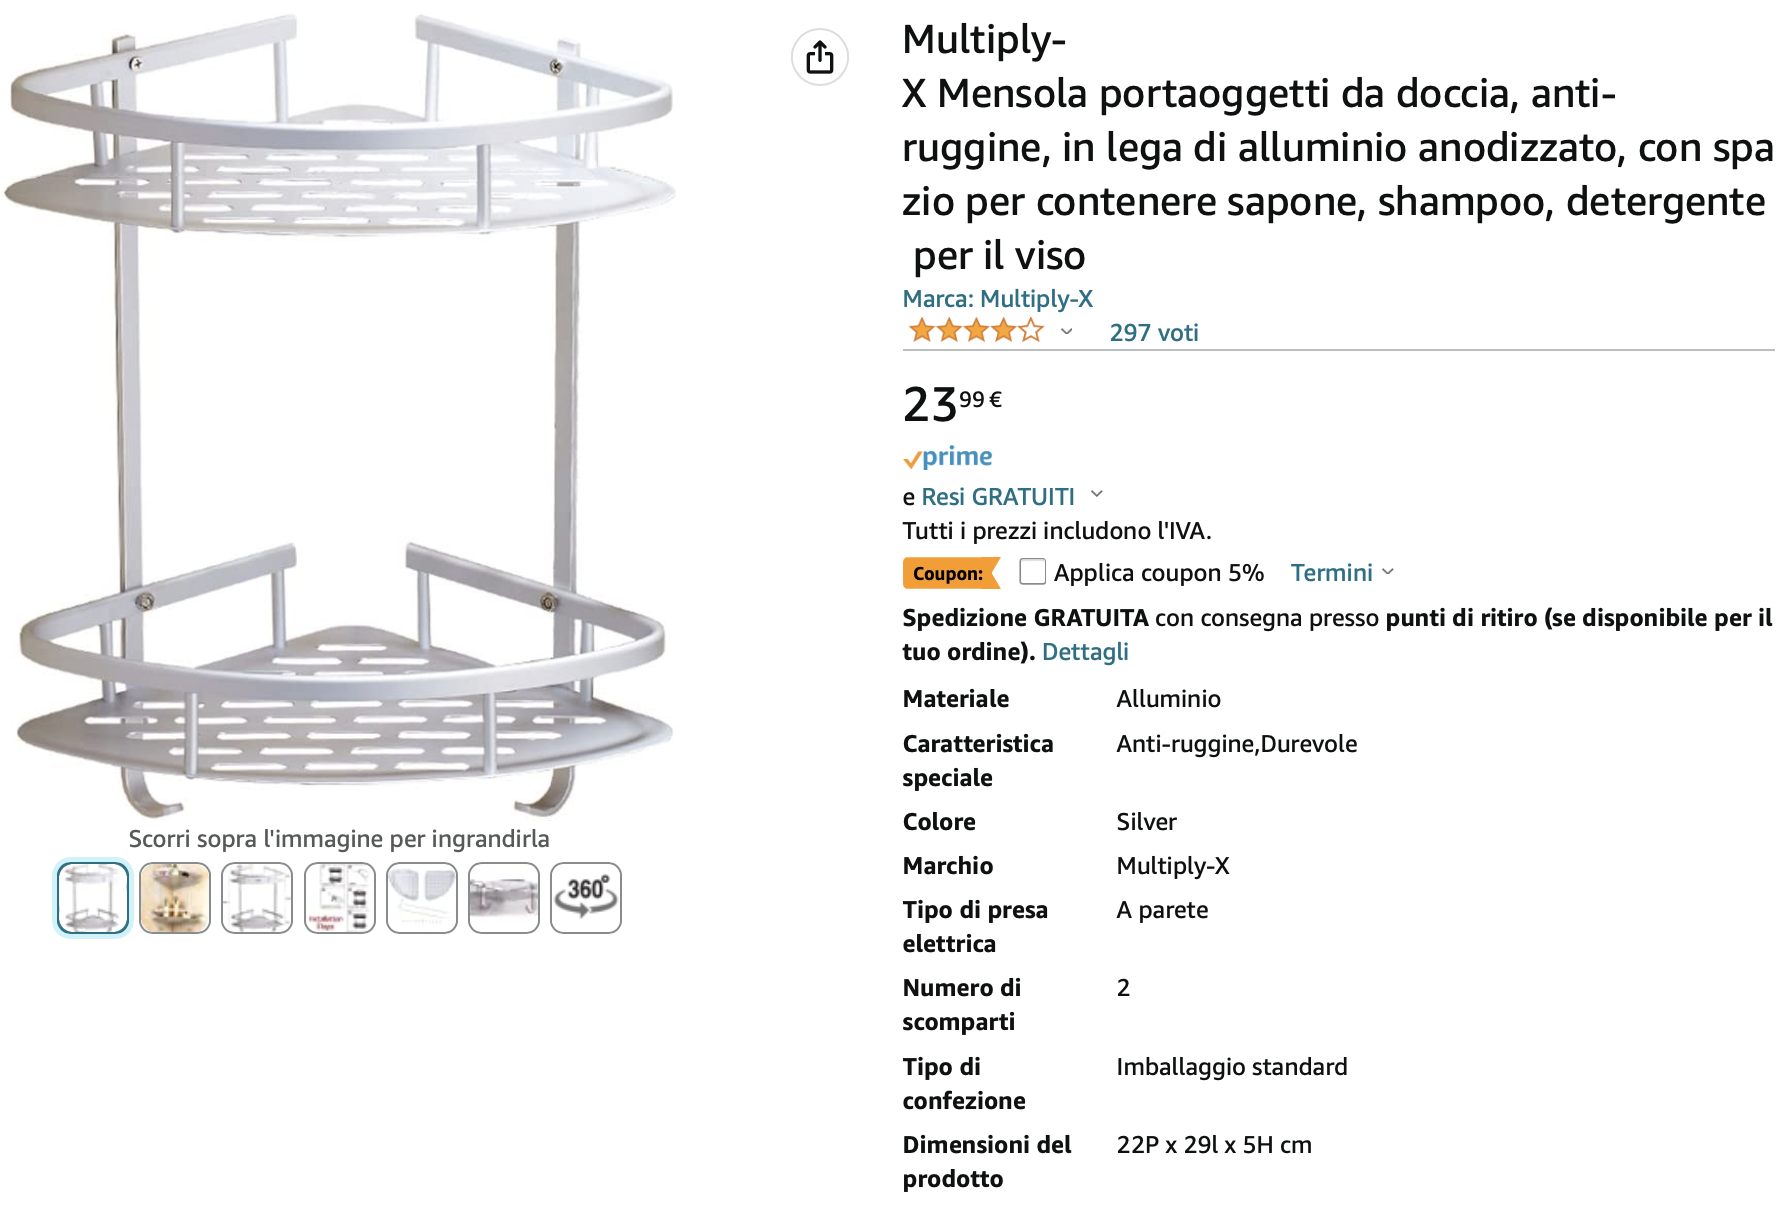
\includegraphics[width=\textwidth, scale=0.2]{img/prod9.png}
%     \caption{Caption}
%     \label{fig:my_label}
% \end{figure}
% \begin{table}[h]
%     \begin{tabular}{|c|c|}
%         \hline
%         \textbf{Materiale} & \\
%         \hline
%         \textbf{Colore} & \\
%         \hline
%         \textbf{Marchio} & \\
%         \hline
%         \textbf{Numero di scomparti} & \\
%         \hline
%         \textbf{Forma} & \\
%         \hline
%     \end{tabular}
%     \caption{Espressioni usate per le restanti caratteristiche}
%     \label{tab:my_label}
% \end{table}

% \subsection{Decimo prodotto}
% \begin{figure}[h]
%     \centering
%     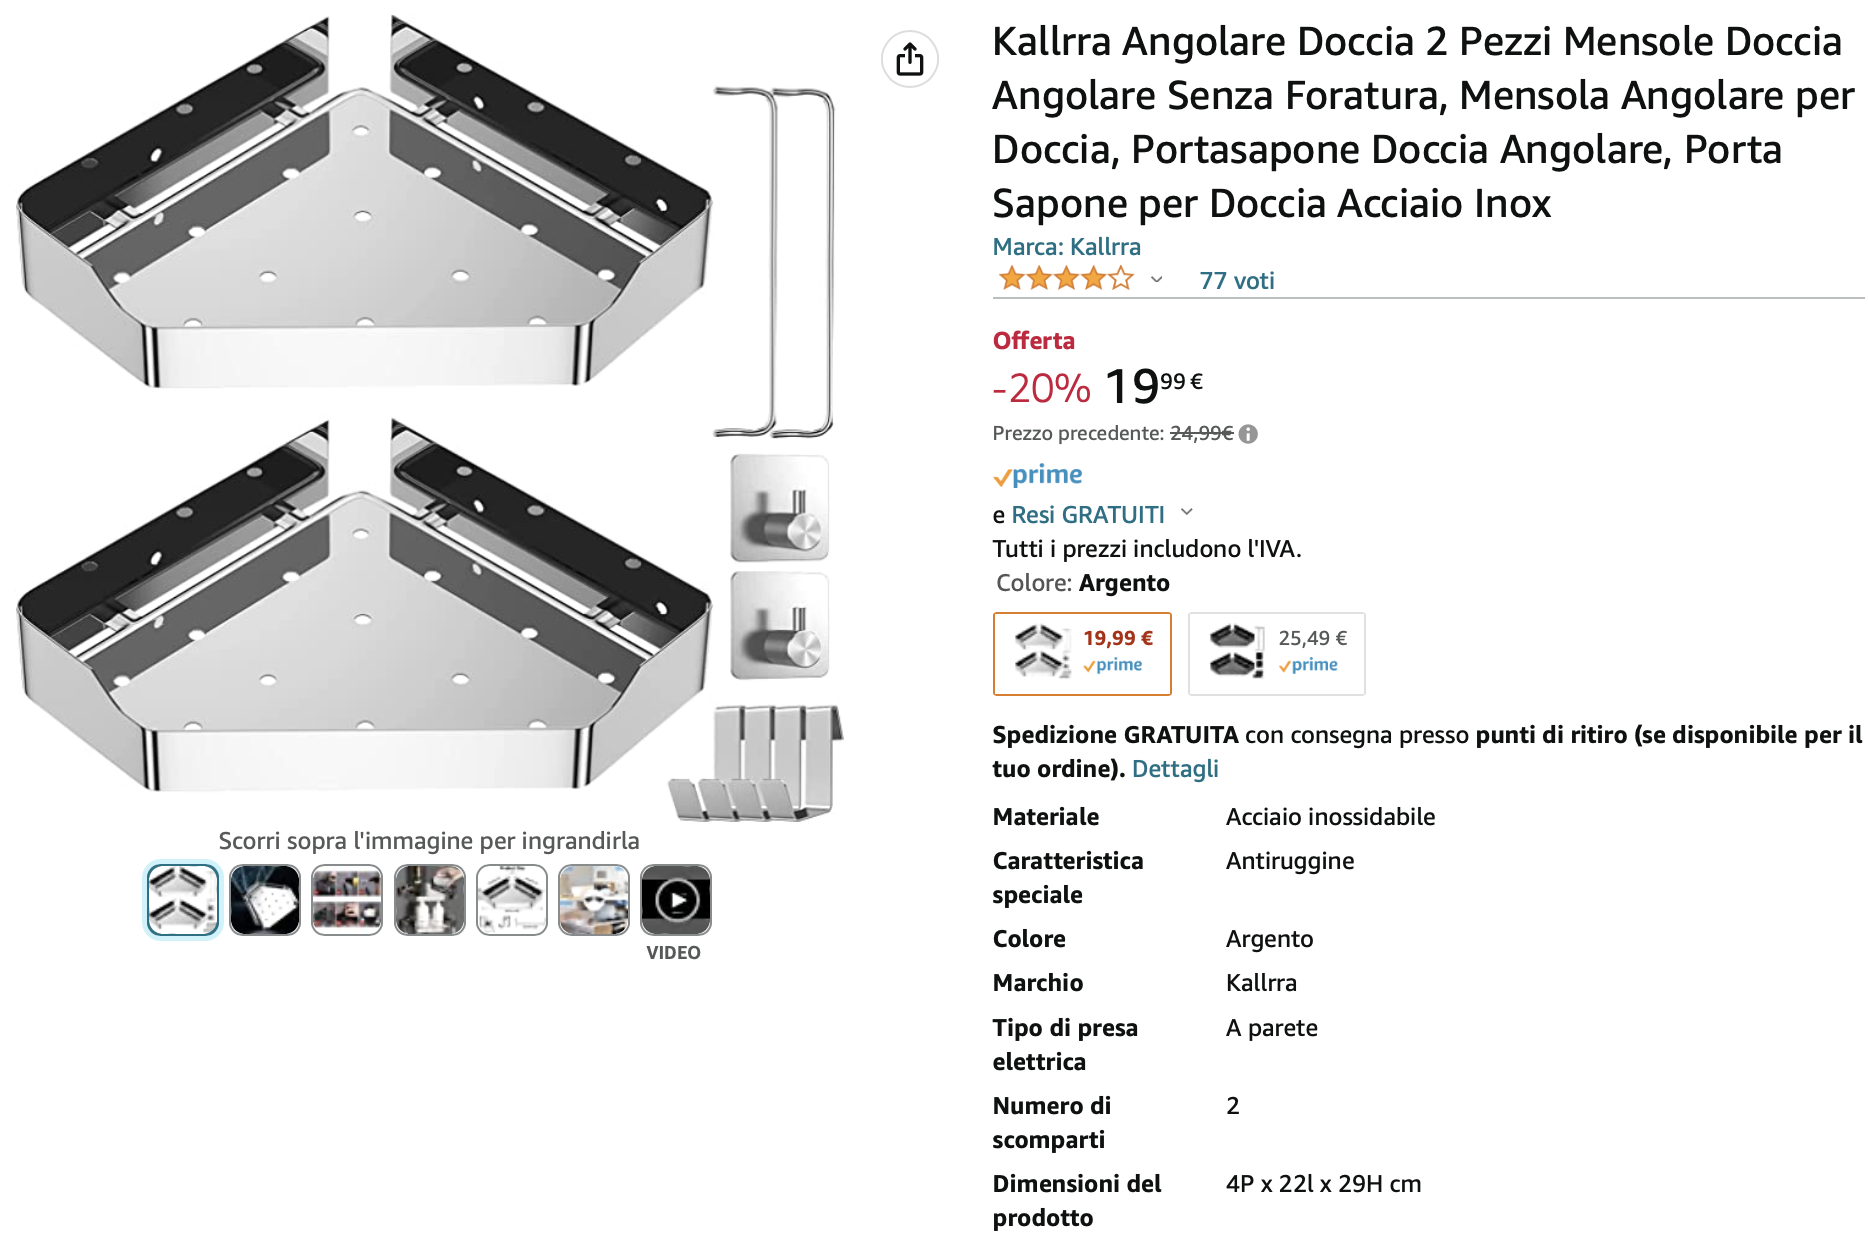
\includegraphics[width=\textwidth, scale=0.2]{img/prod10.png}
%     \caption{Caption}
%     \label{fig:my_label}
% \end{figure}
% \begin{table}[h]
%     \begin{tabular}{|c|c|}
%         \hline
%         \textbf{Materiale} & \\
%         \hline
%         \textbf{Colore} & \\
%         \hline
%         \textbf{Marchio} & \\
%         \hline
%         \textbf{Numero di scomparti} & \\
%         \hline
%         \textbf{Forma} & \\
%         \hline
%     \end{tabular}
%     \caption{Espressioni usate per le restanti caratteristiche}
%     \label{tab:my_label}
% \end{table}